
% Default to the notebook output style

    


% Inherit from the specified cell style.




    
\documentclass[11pt]{article}

    
    
    \usepackage[T1]{fontenc}
    % Nicer default font (+ math font) than Computer Modern for most use cases
    \usepackage{mathpazo}

    % Basic figure setup, for now with no caption control since it's done
    % automatically by Pandoc (which extracts ![](path) syntax from Markdown).
    \usepackage{graphicx}
    % We will generate all images so they have a width \maxwidth. This means
    % that they will get their normal width if they fit onto the page, but
    % are scaled down if they would overflow the margins.
    \makeatletter
    \def\maxwidth{\ifdim\Gin@nat@width>\linewidth\linewidth
    \else\Gin@nat@width\fi}
    \makeatother
    \let\Oldincludegraphics\includegraphics
    % Set max figure width to be 80% of text width, for now hardcoded.
    \renewcommand{\includegraphics}[1]{\Oldincludegraphics[width=.8\maxwidth]{#1}}
    % Ensure that by default, figures have no caption (until we provide a
    % proper Figure object with a Caption API and a way to capture that
    % in the conversion process - todo).
    \usepackage{caption}
    \DeclareCaptionLabelFormat{nolabel}{}
    \captionsetup{labelformat=nolabel}

    \usepackage{adjustbox} % Used to constrain images to a maximum size 
    \usepackage{xcolor} % Allow colors to be defined
    \usepackage{enumerate} % Needed for markdown enumerations to work
    \usepackage{geometry} % Used to adjust the document margins
    \usepackage{amsmath} % Equations
    \usepackage{amssymb} % Equations
    \usepackage{textcomp} % defines textquotesingle
    % Hack from http://tex.stackexchange.com/a/47451/13684:
    \AtBeginDocument{%
        \def\PYZsq{\textquotesingle}% Upright quotes in Pygmentized code
    }
    \usepackage{upquote} % Upright quotes for verbatim code
    \usepackage{eurosym} % defines \euro
    \usepackage[mathletters]{ucs} % Extended unicode (utf-8) support
    \usepackage[utf8x]{inputenc} % Allow utf-8 characters in the tex document
    \usepackage{fancyvrb} % verbatim replacement that allows latex
    \usepackage{grffile} % extends the file name processing of package graphics 
                         % to support a larger range 
    % The hyperref package gives us a pdf with properly built
    % internal navigation ('pdf bookmarks' for the table of contents,
    % internal cross-reference links, web links for URLs, etc.)
    \usepackage{hyperref}
    \usepackage{longtable} % longtable support required by pandoc >1.10
    \usepackage{booktabs}  % table support for pandoc > 1.12.2
    \usepackage[inline]{enumitem} % IRkernel/repr support (it uses the enumerate* environment)
    \usepackage[normalem]{ulem} % ulem is needed to support strikethroughs (\sout)
                                % normalem makes italics be italics, not underlines
    

    
    
    % Colors for the hyperref package
    \definecolor{urlcolor}{rgb}{0,.145,.698}
    \definecolor{linkcolor}{rgb}{.71,0.21,0.01}
    \definecolor{citecolor}{rgb}{.12,.54,.11}

    % ANSI colors
    \definecolor{ansi-black}{HTML}{3E424D}
    \definecolor{ansi-black-intense}{HTML}{282C36}
    \definecolor{ansi-red}{HTML}{E75C58}
    \definecolor{ansi-red-intense}{HTML}{B22B31}
    \definecolor{ansi-green}{HTML}{00A250}
    \definecolor{ansi-green-intense}{HTML}{007427}
    \definecolor{ansi-yellow}{HTML}{DDB62B}
    \definecolor{ansi-yellow-intense}{HTML}{B27D12}
    \definecolor{ansi-blue}{HTML}{208FFB}
    \definecolor{ansi-blue-intense}{HTML}{0065CA}
    \definecolor{ansi-magenta}{HTML}{D160C4}
    \definecolor{ansi-magenta-intense}{HTML}{A03196}
    \definecolor{ansi-cyan}{HTML}{60C6C8}
    \definecolor{ansi-cyan-intense}{HTML}{258F8F}
    \definecolor{ansi-white}{HTML}{C5C1B4}
    \definecolor{ansi-white-intense}{HTML}{A1A6B2}

    % commands and environments needed by pandoc snippets
    % extracted from the output of `pandoc -s`
    \providecommand{\tightlist}{%
      \setlength{\itemsep}{0pt}\setlength{\parskip}{0pt}}
    \DefineVerbatimEnvironment{Highlighting}{Verbatim}{commandchars=\\\{\}}
    % Add ',fontsize=\small' for more characters per line
    \newenvironment{Shaded}{}{}
    \newcommand{\KeywordTok}[1]{\textcolor[rgb]{0.00,0.44,0.13}{\textbf{{#1}}}}
    \newcommand{\DataTypeTok}[1]{\textcolor[rgb]{0.56,0.13,0.00}{{#1}}}
    \newcommand{\DecValTok}[1]{\textcolor[rgb]{0.25,0.63,0.44}{{#1}}}
    \newcommand{\BaseNTok}[1]{\textcolor[rgb]{0.25,0.63,0.44}{{#1}}}
    \newcommand{\FloatTok}[1]{\textcolor[rgb]{0.25,0.63,0.44}{{#1}}}
    \newcommand{\CharTok}[1]{\textcolor[rgb]{0.25,0.44,0.63}{{#1}}}
    \newcommand{\StringTok}[1]{\textcolor[rgb]{0.25,0.44,0.63}{{#1}}}
    \newcommand{\CommentTok}[1]{\textcolor[rgb]{0.38,0.63,0.69}{\textit{{#1}}}}
    \newcommand{\OtherTok}[1]{\textcolor[rgb]{0.00,0.44,0.13}{{#1}}}
    \newcommand{\AlertTok}[1]{\textcolor[rgb]{1.00,0.00,0.00}{\textbf{{#1}}}}
    \newcommand{\FunctionTok}[1]{\textcolor[rgb]{0.02,0.16,0.49}{{#1}}}
    \newcommand{\RegionMarkerTok}[1]{{#1}}
    \newcommand{\ErrorTok}[1]{\textcolor[rgb]{1.00,0.00,0.00}{\textbf{{#1}}}}
    \newcommand{\NormalTok}[1]{{#1}}
    
    % Additional commands for more recent versions of Pandoc
    \newcommand{\ConstantTok}[1]{\textcolor[rgb]{0.53,0.00,0.00}{{#1}}}
    \newcommand{\SpecialCharTok}[1]{\textcolor[rgb]{0.25,0.44,0.63}{{#1}}}
    \newcommand{\VerbatimStringTok}[1]{\textcolor[rgb]{0.25,0.44,0.63}{{#1}}}
    \newcommand{\SpecialStringTok}[1]{\textcolor[rgb]{0.73,0.40,0.53}{{#1}}}
    \newcommand{\ImportTok}[1]{{#1}}
    \newcommand{\DocumentationTok}[1]{\textcolor[rgb]{0.73,0.13,0.13}{\textit{{#1}}}}
    \newcommand{\AnnotationTok}[1]{\textcolor[rgb]{0.38,0.63,0.69}{\textbf{\textit{{#1}}}}}
    \newcommand{\CommentVarTok}[1]{\textcolor[rgb]{0.38,0.63,0.69}{\textbf{\textit{{#1}}}}}
    \newcommand{\VariableTok}[1]{\textcolor[rgb]{0.10,0.09,0.49}{{#1}}}
    \newcommand{\ControlFlowTok}[1]{\textcolor[rgb]{0.00,0.44,0.13}{\textbf{{#1}}}}
    \newcommand{\OperatorTok}[1]{\textcolor[rgb]{0.40,0.40,0.40}{{#1}}}
    \newcommand{\BuiltInTok}[1]{{#1}}
    \newcommand{\ExtensionTok}[1]{{#1}}
    \newcommand{\PreprocessorTok}[1]{\textcolor[rgb]{0.74,0.48,0.00}{{#1}}}
    \newcommand{\AttributeTok}[1]{\textcolor[rgb]{0.49,0.56,0.16}{{#1}}}
    \newcommand{\InformationTok}[1]{\textcolor[rgb]{0.38,0.63,0.69}{\textbf{\textit{{#1}}}}}
    \newcommand{\WarningTok}[1]{\textcolor[rgb]{0.38,0.63,0.69}{\textbf{\textit{{#1}}}}}
    
    
    % Define a nice break command that doesn't care if a line doesn't already
    % exist.
    \def\br{\hspace*{\fill} \\* }
    % Math Jax compatability definitions
    \def\gt{>}
    \def\lt{<}
    % Document parameters
    \title{machine\_translation}
    
    
    

    % Pygments definitions
    
\makeatletter
\def\PY@reset{\let\PY@it=\relax \let\PY@bf=\relax%
    \let\PY@ul=\relax \let\PY@tc=\relax%
    \let\PY@bc=\relax \let\PY@ff=\relax}
\def\PY@tok#1{\csname PY@tok@#1\endcsname}
\def\PY@toks#1+{\ifx\relax#1\empty\else%
    \PY@tok{#1}\expandafter\PY@toks\fi}
\def\PY@do#1{\PY@bc{\PY@tc{\PY@ul{%
    \PY@it{\PY@bf{\PY@ff{#1}}}}}}}
\def\PY#1#2{\PY@reset\PY@toks#1+\relax+\PY@do{#2}}

\expandafter\def\csname PY@tok@w\endcsname{\def\PY@tc##1{\textcolor[rgb]{0.73,0.73,0.73}{##1}}}
\expandafter\def\csname PY@tok@c\endcsname{\let\PY@it=\textit\def\PY@tc##1{\textcolor[rgb]{0.25,0.50,0.50}{##1}}}
\expandafter\def\csname PY@tok@cp\endcsname{\def\PY@tc##1{\textcolor[rgb]{0.74,0.48,0.00}{##1}}}
\expandafter\def\csname PY@tok@k\endcsname{\let\PY@bf=\textbf\def\PY@tc##1{\textcolor[rgb]{0.00,0.50,0.00}{##1}}}
\expandafter\def\csname PY@tok@kp\endcsname{\def\PY@tc##1{\textcolor[rgb]{0.00,0.50,0.00}{##1}}}
\expandafter\def\csname PY@tok@kt\endcsname{\def\PY@tc##1{\textcolor[rgb]{0.69,0.00,0.25}{##1}}}
\expandafter\def\csname PY@tok@o\endcsname{\def\PY@tc##1{\textcolor[rgb]{0.40,0.40,0.40}{##1}}}
\expandafter\def\csname PY@tok@ow\endcsname{\let\PY@bf=\textbf\def\PY@tc##1{\textcolor[rgb]{0.67,0.13,1.00}{##1}}}
\expandafter\def\csname PY@tok@nb\endcsname{\def\PY@tc##1{\textcolor[rgb]{0.00,0.50,0.00}{##1}}}
\expandafter\def\csname PY@tok@nf\endcsname{\def\PY@tc##1{\textcolor[rgb]{0.00,0.00,1.00}{##1}}}
\expandafter\def\csname PY@tok@nc\endcsname{\let\PY@bf=\textbf\def\PY@tc##1{\textcolor[rgb]{0.00,0.00,1.00}{##1}}}
\expandafter\def\csname PY@tok@nn\endcsname{\let\PY@bf=\textbf\def\PY@tc##1{\textcolor[rgb]{0.00,0.00,1.00}{##1}}}
\expandafter\def\csname PY@tok@ne\endcsname{\let\PY@bf=\textbf\def\PY@tc##1{\textcolor[rgb]{0.82,0.25,0.23}{##1}}}
\expandafter\def\csname PY@tok@nv\endcsname{\def\PY@tc##1{\textcolor[rgb]{0.10,0.09,0.49}{##1}}}
\expandafter\def\csname PY@tok@no\endcsname{\def\PY@tc##1{\textcolor[rgb]{0.53,0.00,0.00}{##1}}}
\expandafter\def\csname PY@tok@nl\endcsname{\def\PY@tc##1{\textcolor[rgb]{0.63,0.63,0.00}{##1}}}
\expandafter\def\csname PY@tok@ni\endcsname{\let\PY@bf=\textbf\def\PY@tc##1{\textcolor[rgb]{0.60,0.60,0.60}{##1}}}
\expandafter\def\csname PY@tok@na\endcsname{\def\PY@tc##1{\textcolor[rgb]{0.49,0.56,0.16}{##1}}}
\expandafter\def\csname PY@tok@nt\endcsname{\let\PY@bf=\textbf\def\PY@tc##1{\textcolor[rgb]{0.00,0.50,0.00}{##1}}}
\expandafter\def\csname PY@tok@nd\endcsname{\def\PY@tc##1{\textcolor[rgb]{0.67,0.13,1.00}{##1}}}
\expandafter\def\csname PY@tok@s\endcsname{\def\PY@tc##1{\textcolor[rgb]{0.73,0.13,0.13}{##1}}}
\expandafter\def\csname PY@tok@sd\endcsname{\let\PY@it=\textit\def\PY@tc##1{\textcolor[rgb]{0.73,0.13,0.13}{##1}}}
\expandafter\def\csname PY@tok@si\endcsname{\let\PY@bf=\textbf\def\PY@tc##1{\textcolor[rgb]{0.73,0.40,0.53}{##1}}}
\expandafter\def\csname PY@tok@se\endcsname{\let\PY@bf=\textbf\def\PY@tc##1{\textcolor[rgb]{0.73,0.40,0.13}{##1}}}
\expandafter\def\csname PY@tok@sr\endcsname{\def\PY@tc##1{\textcolor[rgb]{0.73,0.40,0.53}{##1}}}
\expandafter\def\csname PY@tok@ss\endcsname{\def\PY@tc##1{\textcolor[rgb]{0.10,0.09,0.49}{##1}}}
\expandafter\def\csname PY@tok@sx\endcsname{\def\PY@tc##1{\textcolor[rgb]{0.00,0.50,0.00}{##1}}}
\expandafter\def\csname PY@tok@m\endcsname{\def\PY@tc##1{\textcolor[rgb]{0.40,0.40,0.40}{##1}}}
\expandafter\def\csname PY@tok@gh\endcsname{\let\PY@bf=\textbf\def\PY@tc##1{\textcolor[rgb]{0.00,0.00,0.50}{##1}}}
\expandafter\def\csname PY@tok@gu\endcsname{\let\PY@bf=\textbf\def\PY@tc##1{\textcolor[rgb]{0.50,0.00,0.50}{##1}}}
\expandafter\def\csname PY@tok@gd\endcsname{\def\PY@tc##1{\textcolor[rgb]{0.63,0.00,0.00}{##1}}}
\expandafter\def\csname PY@tok@gi\endcsname{\def\PY@tc##1{\textcolor[rgb]{0.00,0.63,0.00}{##1}}}
\expandafter\def\csname PY@tok@gr\endcsname{\def\PY@tc##1{\textcolor[rgb]{1.00,0.00,0.00}{##1}}}
\expandafter\def\csname PY@tok@ge\endcsname{\let\PY@it=\textit}
\expandafter\def\csname PY@tok@gs\endcsname{\let\PY@bf=\textbf}
\expandafter\def\csname PY@tok@gp\endcsname{\let\PY@bf=\textbf\def\PY@tc##1{\textcolor[rgb]{0.00,0.00,0.50}{##1}}}
\expandafter\def\csname PY@tok@go\endcsname{\def\PY@tc##1{\textcolor[rgb]{0.53,0.53,0.53}{##1}}}
\expandafter\def\csname PY@tok@gt\endcsname{\def\PY@tc##1{\textcolor[rgb]{0.00,0.27,0.87}{##1}}}
\expandafter\def\csname PY@tok@err\endcsname{\def\PY@bc##1{\setlength{\fboxsep}{0pt}\fcolorbox[rgb]{1.00,0.00,0.00}{1,1,1}{\strut ##1}}}
\expandafter\def\csname PY@tok@kc\endcsname{\let\PY@bf=\textbf\def\PY@tc##1{\textcolor[rgb]{0.00,0.50,0.00}{##1}}}
\expandafter\def\csname PY@tok@kd\endcsname{\let\PY@bf=\textbf\def\PY@tc##1{\textcolor[rgb]{0.00,0.50,0.00}{##1}}}
\expandafter\def\csname PY@tok@kn\endcsname{\let\PY@bf=\textbf\def\PY@tc##1{\textcolor[rgb]{0.00,0.50,0.00}{##1}}}
\expandafter\def\csname PY@tok@kr\endcsname{\let\PY@bf=\textbf\def\PY@tc##1{\textcolor[rgb]{0.00,0.50,0.00}{##1}}}
\expandafter\def\csname PY@tok@bp\endcsname{\def\PY@tc##1{\textcolor[rgb]{0.00,0.50,0.00}{##1}}}
\expandafter\def\csname PY@tok@fm\endcsname{\def\PY@tc##1{\textcolor[rgb]{0.00,0.00,1.00}{##1}}}
\expandafter\def\csname PY@tok@vc\endcsname{\def\PY@tc##1{\textcolor[rgb]{0.10,0.09,0.49}{##1}}}
\expandafter\def\csname PY@tok@vg\endcsname{\def\PY@tc##1{\textcolor[rgb]{0.10,0.09,0.49}{##1}}}
\expandafter\def\csname PY@tok@vi\endcsname{\def\PY@tc##1{\textcolor[rgb]{0.10,0.09,0.49}{##1}}}
\expandafter\def\csname PY@tok@vm\endcsname{\def\PY@tc##1{\textcolor[rgb]{0.10,0.09,0.49}{##1}}}
\expandafter\def\csname PY@tok@sa\endcsname{\def\PY@tc##1{\textcolor[rgb]{0.73,0.13,0.13}{##1}}}
\expandafter\def\csname PY@tok@sb\endcsname{\def\PY@tc##1{\textcolor[rgb]{0.73,0.13,0.13}{##1}}}
\expandafter\def\csname PY@tok@sc\endcsname{\def\PY@tc##1{\textcolor[rgb]{0.73,0.13,0.13}{##1}}}
\expandafter\def\csname PY@tok@dl\endcsname{\def\PY@tc##1{\textcolor[rgb]{0.73,0.13,0.13}{##1}}}
\expandafter\def\csname PY@tok@s2\endcsname{\def\PY@tc##1{\textcolor[rgb]{0.73,0.13,0.13}{##1}}}
\expandafter\def\csname PY@tok@sh\endcsname{\def\PY@tc##1{\textcolor[rgb]{0.73,0.13,0.13}{##1}}}
\expandafter\def\csname PY@tok@s1\endcsname{\def\PY@tc##1{\textcolor[rgb]{0.73,0.13,0.13}{##1}}}
\expandafter\def\csname PY@tok@mb\endcsname{\def\PY@tc##1{\textcolor[rgb]{0.40,0.40,0.40}{##1}}}
\expandafter\def\csname PY@tok@mf\endcsname{\def\PY@tc##1{\textcolor[rgb]{0.40,0.40,0.40}{##1}}}
\expandafter\def\csname PY@tok@mh\endcsname{\def\PY@tc##1{\textcolor[rgb]{0.40,0.40,0.40}{##1}}}
\expandafter\def\csname PY@tok@mi\endcsname{\def\PY@tc##1{\textcolor[rgb]{0.40,0.40,0.40}{##1}}}
\expandafter\def\csname PY@tok@il\endcsname{\def\PY@tc##1{\textcolor[rgb]{0.40,0.40,0.40}{##1}}}
\expandafter\def\csname PY@tok@mo\endcsname{\def\PY@tc##1{\textcolor[rgb]{0.40,0.40,0.40}{##1}}}
\expandafter\def\csname PY@tok@ch\endcsname{\let\PY@it=\textit\def\PY@tc##1{\textcolor[rgb]{0.25,0.50,0.50}{##1}}}
\expandafter\def\csname PY@tok@cm\endcsname{\let\PY@it=\textit\def\PY@tc##1{\textcolor[rgb]{0.25,0.50,0.50}{##1}}}
\expandafter\def\csname PY@tok@cpf\endcsname{\let\PY@it=\textit\def\PY@tc##1{\textcolor[rgb]{0.25,0.50,0.50}{##1}}}
\expandafter\def\csname PY@tok@c1\endcsname{\let\PY@it=\textit\def\PY@tc##1{\textcolor[rgb]{0.25,0.50,0.50}{##1}}}
\expandafter\def\csname PY@tok@cs\endcsname{\let\PY@it=\textit\def\PY@tc##1{\textcolor[rgb]{0.25,0.50,0.50}{##1}}}

\def\PYZbs{\char`\\}
\def\PYZus{\char`\_}
\def\PYZob{\char`\{}
\def\PYZcb{\char`\}}
\def\PYZca{\char`\^}
\def\PYZam{\char`\&}
\def\PYZlt{\char`\<}
\def\PYZgt{\char`\>}
\def\PYZsh{\char`\#}
\def\PYZpc{\char`\%}
\def\PYZdl{\char`\$}
\def\PYZhy{\char`\-}
\def\PYZsq{\char`\'}
\def\PYZdq{\char`\"}
\def\PYZti{\char`\~}
% for compatibility with earlier versions
\def\PYZat{@}
\def\PYZlb{[}
\def\PYZrb{]}
\makeatother


    % Exact colors from NB
    \definecolor{incolor}{rgb}{0.0, 0.0, 0.5}
    \definecolor{outcolor}{rgb}{0.545, 0.0, 0.0}



    
    % Prevent overflowing lines due to hard-to-break entities
    \sloppy 
    % Setup hyperref package
    \hypersetup{
      breaklinks=true,  % so long urls are correctly broken across lines
      colorlinks=true,
      urlcolor=urlcolor,
      linkcolor=linkcolor,
      citecolor=citecolor,
      }
    % Slightly bigger margins than the latex defaults
    
    \geometry{verbose,tmargin=1in,bmargin=1in,lmargin=1in,rmargin=1in}
    
    

    \begin{document}
    
    
    \maketitle
    
    

    
    \section{Artificial Intelligence
Nanodegree}\label{artificial-intelligence-nanodegree}

\subsection{Machine Translation
Project}\label{machine-translation-project}

In this notebook, sections that end with \textbf{'(IMPLEMENTATION)'} in
the header indicate that the following blocks of code will require
additional functionality which you must provide. Please be sure to read
the instructions carefully!

\subsection{Introduction}\label{introduction}

In this notebook, you will build a deep neural network that functions as
part of an end-to-end machine translation pipeline. Your completed
pipeline will accept English text as input and return the French
translation.

\begin{itemize}
\tightlist
\item
  \textbf{Preprocess} - You'll convert text to sequence of integers.
\item
  \textbf{Models} Create models which accepts a sequence of integers as
  input and returns a probability distribution over possible
  translations. After learning about the basic types of neural networks
  that are often used for machine translation, you will engage in your
  own investigations, to design your own model!
\item
  \textbf{Prediction} Run the model on English text.
\end{itemize}

    \begin{Verbatim}[commandchars=\\\{\}]
{\color{incolor}In [{\color{incolor}1}]:} \PY{o}{\PYZpc{}}\PY{k}{load\PYZus{}ext} autoreload
        \PY{o}{\PYZpc{}}\PY{k}{aimport} helper, tests
        \PY{o}{\PYZpc{}}\PY{k}{autoreload} 1
\end{Verbatim}


    \begin{Verbatim}[commandchars=\\\{\}]
{\color{incolor}In [{\color{incolor}2}]:} \PY{k+kn}{import} \PY{n+nn}{collections}
        
        \PY{k+kn}{import} \PY{n+nn}{helper}
        \PY{k+kn}{import} \PY{n+nn}{numpy} \PY{k}{as} \PY{n+nn}{np}
        \PY{k+kn}{import} \PY{n+nn}{project\PYZus{}tests} \PY{k}{as} \PY{n+nn}{tests}
        
        \PY{k+kn}{from} \PY{n+nn}{keras}\PY{n+nn}{.}\PY{n+nn}{preprocessing}\PY{n+nn}{.}\PY{n+nn}{text} \PY{k}{import} \PY{n}{Tokenizer}
        \PY{k+kn}{from} \PY{n+nn}{keras}\PY{n+nn}{.}\PY{n+nn}{preprocessing}\PY{n+nn}{.}\PY{n+nn}{sequence} \PY{k}{import} \PY{n}{pad\PYZus{}sequences}
        \PY{k+kn}{from} \PY{n+nn}{keras}\PY{n+nn}{.}\PY{n+nn}{models} \PY{k}{import} \PY{n}{Model}\PY{p}{,} \PY{n}{Sequential}
        \PY{k+kn}{from} \PY{n+nn}{keras}\PY{n+nn}{.}\PY{n+nn}{layers} \PY{k}{import} \PY{n}{GRU}\PY{p}{,} \PY{n}{Input}\PY{p}{,} \PY{n}{Dense}\PY{p}{,} \PY{n}{TimeDistributed}\PY{p}{,} \PY{n}{Activation}\PY{p}{,} \PY{n}{RepeatVector}\PY{p}{,} \PY{n}{Bidirectional}\PY{p}{,} \PY{n}{LSTM}
        \PY{k+kn}{from} \PY{n+nn}{keras}\PY{n+nn}{.}\PY{n+nn}{layers}\PY{n+nn}{.}\PY{n+nn}{embeddings} \PY{k}{import} \PY{n}{Embedding}
        \PY{k+kn}{from} \PY{n+nn}{keras}\PY{n+nn}{.}\PY{n+nn}{optimizers} \PY{k}{import} \PY{n}{Adam}
        \PY{k+kn}{from} \PY{n+nn}{keras}\PY{n+nn}{.}\PY{n+nn}{losses} \PY{k}{import} \PY{n}{sparse\PYZus{}categorical\PYZus{}crossentropy}
\end{Verbatim}


    \begin{Verbatim}[commandchars=\\\{\}]
Using TensorFlow backend.

    \end{Verbatim}

    \subsubsection{Verify access to the GPU}\label{verify-access-to-the-gpu}

The following test applies only if you expect to be using a GPU, e.g.,
while running in a Udacity Workspace or using an AWS instance with GPU
support. Run the next cell, and verify that the device\_type is "GPU". -
If the device is not GPU \& you are running from a Udacity Workspace,
then save your workspace with the icon at the top, then click "enable"
at the bottom of the workspace. - If the device is not GPU \& you are
running from an AWS instance, then refer to the cloud computing
instructions in the classroom to verify your setup steps.

    \begin{Verbatim}[commandchars=\\\{\}]
{\color{incolor}In [{\color{incolor}3}]:} \PY{k+kn}{from} \PY{n+nn}{tensorflow}\PY{n+nn}{.}\PY{n+nn}{python}\PY{n+nn}{.}\PY{n+nn}{client} \PY{k}{import} \PY{n}{device\PYZus{}lib}
        \PY{n+nb}{print}\PY{p}{(}\PY{n}{device\PYZus{}lib}\PY{o}{.}\PY{n}{list\PYZus{}local\PYZus{}devices}\PY{p}{(}\PY{p}{)}\PY{p}{)}
\end{Verbatim}


    \begin{Verbatim}[commandchars=\\\{\}]
[name: "/cpu:0"
device\_type: "CPU"
memory\_limit: 268435456
locality \{
\}
incarnation: 2688222564311024193
, name: "/gpu:0"
device\_type: "GPU"
memory\_limit: 357302272
locality \{
  bus\_id: 1
\}
incarnation: 13538233064103867964
physical\_device\_desc: "device: 0, name: Tesla K80, pci bus id: 0000:00:04.0"
]

    \end{Verbatim}

    \subsection{Dataset}\label{dataset}

We begin by investigating the dataset that will be used to train and
evaluate your pipeline. The most common datasets used for machine
translation are from \href{http://www.statmt.org/}{WMT}. However, that
will take a long time to train a neural network on. We'll be using a
dataset we created for this project that contains a small vocabulary.
You'll be able to train your model in a reasonable time with this
dataset. \#\#\# Load Data The data is located in
\texttt{data/small\_vocab\_en} and \texttt{data/small\_vocab\_fr}. The
\texttt{small\_vocab\_en} file contains English sentences with their
French translations in the \texttt{small\_vocab\_fr} file. Load the
English and French data from these files from running the cell below.

    \begin{Verbatim}[commandchars=\\\{\}]
{\color{incolor}In [{\color{incolor}4}]:} \PY{c+c1}{\PYZsh{} Load English data}
        \PY{n}{english\PYZus{}sentences} \PY{o}{=} \PY{n}{helper}\PY{o}{.}\PY{n}{load\PYZus{}data}\PY{p}{(}\PY{l+s+s1}{\PYZsq{}}\PY{l+s+s1}{data/small\PYZus{}vocab\PYZus{}en}\PY{l+s+s1}{\PYZsq{}}\PY{p}{)}
        \PY{c+c1}{\PYZsh{} Load French data}
        \PY{n}{french\PYZus{}sentences} \PY{o}{=} \PY{n}{helper}\PY{o}{.}\PY{n}{load\PYZus{}data}\PY{p}{(}\PY{l+s+s1}{\PYZsq{}}\PY{l+s+s1}{data/small\PYZus{}vocab\PYZus{}fr}\PY{l+s+s1}{\PYZsq{}}\PY{p}{)}
        
        \PY{n+nb}{print}\PY{p}{(}\PY{l+s+s1}{\PYZsq{}}\PY{l+s+s1}{Dataset Loaded}\PY{l+s+s1}{\PYZsq{}}\PY{p}{)}
\end{Verbatim}


    \begin{Verbatim}[commandchars=\\\{\}]
Dataset Loaded

    \end{Verbatim}

    \subsubsection{Files}\label{files}

Each line in \texttt{small\_vocab\_en} contains an English sentence with
the respective translation in each line of \texttt{small\_vocab\_fr}.
View the first two lines from each file.

    \begin{Verbatim}[commandchars=\\\{\}]
{\color{incolor}In [{\color{incolor}5}]:} \PY{k}{for} \PY{n}{sample\PYZus{}i} \PY{o+ow}{in} \PY{n+nb}{range}\PY{p}{(}\PY{l+m+mi}{2}\PY{p}{)}\PY{p}{:}
            \PY{n+nb}{print}\PY{p}{(}\PY{l+s+s1}{\PYZsq{}}\PY{l+s+s1}{small\PYZus{}vocab\PYZus{}en Line }\PY{l+s+si}{\PYZob{}\PYZcb{}}\PY{l+s+s1}{:  }\PY{l+s+si}{\PYZob{}\PYZcb{}}\PY{l+s+s1}{\PYZsq{}}\PY{o}{.}\PY{n}{format}\PY{p}{(}\PY{n}{sample\PYZus{}i} \PY{o}{+} \PY{l+m+mi}{1}\PY{p}{,} \PY{n}{english\PYZus{}sentences}\PY{p}{[}\PY{n}{sample\PYZus{}i}\PY{p}{]}\PY{p}{)}\PY{p}{)}
            \PY{n+nb}{print}\PY{p}{(}\PY{l+s+s1}{\PYZsq{}}\PY{l+s+s1}{small\PYZus{}vocab\PYZus{}fr Line }\PY{l+s+si}{\PYZob{}\PYZcb{}}\PY{l+s+s1}{:  }\PY{l+s+si}{\PYZob{}\PYZcb{}}\PY{l+s+s1}{\PYZsq{}}\PY{o}{.}\PY{n}{format}\PY{p}{(}\PY{n}{sample\PYZus{}i} \PY{o}{+} \PY{l+m+mi}{1}\PY{p}{,} \PY{n}{french\PYZus{}sentences}\PY{p}{[}\PY{n}{sample\PYZus{}i}\PY{p}{]}\PY{p}{)}\PY{p}{)}
\end{Verbatim}


    \begin{Verbatim}[commandchars=\\\{\}]
small\_vocab\_en Line 1:  new jersey is sometimes quiet during autumn , and it is snowy in april .
small\_vocab\_fr Line 1:  new jersey est parfois calme pendant l' automne , et il est neigeux en avril .
small\_vocab\_en Line 2:  the united states is usually chilly during july , and it is usually freezing in november .
small\_vocab\_fr Line 2:  les états-unis est généralement froid en juillet , et il gèle habituellement en novembre .

    \end{Verbatim}

    From looking at the sentences, you can see they have been preprocessed
already. The puncuations have been delimited using spaces. All the text
has been converted to lowercase. This should save you some time, but the
text requires more preprocessing. \#\#\# Vocabulary The complexity of
the problem is determined by the complexity of the vocabulary. A more
complex vocabulary is a more complex problem. Let's look at the
complexity of the dataset we'll be working with.

    \begin{Verbatim}[commandchars=\\\{\}]
{\color{incolor}In [{\color{incolor}6}]:} \PY{n}{english\PYZus{}words\PYZus{}counter} \PY{o}{=} \PY{n}{collections}\PY{o}{.}\PY{n}{Counter}\PY{p}{(}\PY{p}{[}\PY{n}{word} \PY{k}{for} \PY{n}{sentence} \PY{o+ow}{in} \PY{n}{english\PYZus{}sentences} \PY{k}{for} \PY{n}{word} \PY{o+ow}{in} \PY{n}{sentence}\PY{o}{.}\PY{n}{split}\PY{p}{(}\PY{p}{)}\PY{p}{]}\PY{p}{)}
        \PY{n}{french\PYZus{}words\PYZus{}counter} \PY{o}{=} \PY{n}{collections}\PY{o}{.}\PY{n}{Counter}\PY{p}{(}\PY{p}{[}\PY{n}{word} \PY{k}{for} \PY{n}{sentence} \PY{o+ow}{in} \PY{n}{french\PYZus{}sentences} \PY{k}{for} \PY{n}{word} \PY{o+ow}{in} \PY{n}{sentence}\PY{o}{.}\PY{n}{split}\PY{p}{(}\PY{p}{)}\PY{p}{]}\PY{p}{)}
        
        \PY{n+nb}{print}\PY{p}{(}\PY{l+s+s1}{\PYZsq{}}\PY{l+s+si}{\PYZob{}\PYZcb{}}\PY{l+s+s1}{ English words.}\PY{l+s+s1}{\PYZsq{}}\PY{o}{.}\PY{n}{format}\PY{p}{(}\PY{n+nb}{len}\PY{p}{(}\PY{p}{[}\PY{n}{word} \PY{k}{for} \PY{n}{sentence} \PY{o+ow}{in} \PY{n}{english\PYZus{}sentences} \PY{k}{for} \PY{n}{word} \PY{o+ow}{in} \PY{n}{sentence}\PY{o}{.}\PY{n}{split}\PY{p}{(}\PY{p}{)}\PY{p}{]}\PY{p}{)}\PY{p}{)}\PY{p}{)}
        \PY{n+nb}{print}\PY{p}{(}\PY{l+s+s1}{\PYZsq{}}\PY{l+s+si}{\PYZob{}\PYZcb{}}\PY{l+s+s1}{ unique English words.}\PY{l+s+s1}{\PYZsq{}}\PY{o}{.}\PY{n}{format}\PY{p}{(}\PY{n+nb}{len}\PY{p}{(}\PY{n}{english\PYZus{}words\PYZus{}counter}\PY{p}{)}\PY{p}{)}\PY{p}{)}
        \PY{n+nb}{print}\PY{p}{(}\PY{l+s+s1}{\PYZsq{}}\PY{l+s+s1}{10 Most common words in the English dataset:}\PY{l+s+s1}{\PYZsq{}}\PY{p}{)}
        \PY{n+nb}{print}\PY{p}{(}\PY{l+s+s1}{\PYZsq{}}\PY{l+s+s1}{\PYZdq{}}\PY{l+s+s1}{\PYZsq{}} \PY{o}{+} \PY{l+s+s1}{\PYZsq{}}\PY{l+s+s1}{\PYZdq{}}\PY{l+s+s1}{ }\PY{l+s+s1}{\PYZdq{}}\PY{l+s+s1}{\PYZsq{}}\PY{o}{.}\PY{n}{join}\PY{p}{(}\PY{n+nb}{list}\PY{p}{(}\PY{n+nb}{zip}\PY{p}{(}\PY{o}{*}\PY{n}{english\PYZus{}words\PYZus{}counter}\PY{o}{.}\PY{n}{most\PYZus{}common}\PY{p}{(}\PY{l+m+mi}{10}\PY{p}{)}\PY{p}{)}\PY{p}{)}\PY{p}{[}\PY{l+m+mi}{0}\PY{p}{]}\PY{p}{)} \PY{o}{+} \PY{l+s+s1}{\PYZsq{}}\PY{l+s+s1}{\PYZdq{}}\PY{l+s+s1}{\PYZsq{}}\PY{p}{)}
        \PY{n+nb}{print}\PY{p}{(}\PY{p}{)}
        \PY{n+nb}{print}\PY{p}{(}\PY{l+s+s1}{\PYZsq{}}\PY{l+s+si}{\PYZob{}\PYZcb{}}\PY{l+s+s1}{ French words.}\PY{l+s+s1}{\PYZsq{}}\PY{o}{.}\PY{n}{format}\PY{p}{(}\PY{n+nb}{len}\PY{p}{(}\PY{p}{[}\PY{n}{word} \PY{k}{for} \PY{n}{sentence} \PY{o+ow}{in} \PY{n}{french\PYZus{}sentences} \PY{k}{for} \PY{n}{word} \PY{o+ow}{in} \PY{n}{sentence}\PY{o}{.}\PY{n}{split}\PY{p}{(}\PY{p}{)}\PY{p}{]}\PY{p}{)}\PY{p}{)}\PY{p}{)}
        \PY{n+nb}{print}\PY{p}{(}\PY{l+s+s1}{\PYZsq{}}\PY{l+s+si}{\PYZob{}\PYZcb{}}\PY{l+s+s1}{ unique French words.}\PY{l+s+s1}{\PYZsq{}}\PY{o}{.}\PY{n}{format}\PY{p}{(}\PY{n+nb}{len}\PY{p}{(}\PY{n}{french\PYZus{}words\PYZus{}counter}\PY{p}{)}\PY{p}{)}\PY{p}{)}
        \PY{n+nb}{print}\PY{p}{(}\PY{l+s+s1}{\PYZsq{}}\PY{l+s+s1}{10 Most common words in the French dataset:}\PY{l+s+s1}{\PYZsq{}}\PY{p}{)}
        \PY{n+nb}{print}\PY{p}{(}\PY{l+s+s1}{\PYZsq{}}\PY{l+s+s1}{\PYZdq{}}\PY{l+s+s1}{\PYZsq{}} \PY{o}{+} \PY{l+s+s1}{\PYZsq{}}\PY{l+s+s1}{\PYZdq{}}\PY{l+s+s1}{ }\PY{l+s+s1}{\PYZdq{}}\PY{l+s+s1}{\PYZsq{}}\PY{o}{.}\PY{n}{join}\PY{p}{(}\PY{n+nb}{list}\PY{p}{(}\PY{n+nb}{zip}\PY{p}{(}\PY{o}{*}\PY{n}{french\PYZus{}words\PYZus{}counter}\PY{o}{.}\PY{n}{most\PYZus{}common}\PY{p}{(}\PY{l+m+mi}{10}\PY{p}{)}\PY{p}{)}\PY{p}{)}\PY{p}{[}\PY{l+m+mi}{0}\PY{p}{]}\PY{p}{)} \PY{o}{+} \PY{l+s+s1}{\PYZsq{}}\PY{l+s+s1}{\PYZdq{}}\PY{l+s+s1}{\PYZsq{}}\PY{p}{)}
\end{Verbatim}


    \begin{Verbatim}[commandchars=\\\{\}]
1823250 English words.
227 unique English words.
10 Most common words in the English dataset:
"is" "," "." "in" "it" "during" "the" "but" "and" "sometimes"

1961295 French words.
355 unique French words.
10 Most common words in the French dataset:
"est" "." "," "en" "il" "les" "mais" "et" "la" "parfois"

    \end{Verbatim}

    For comparison, \emph{Alice's Adventures in Wonderland} contains 2,766
unique words of a total of 15,500 words. \#\# Preprocess For this
project, you won't use text data as input to your model. Instead, you'll
convert the text into sequences of integers using the following
preprocess methods: 1. Tokenize the words into ids 2. Add padding to
make all the sequences the same length.

Time to start preprocessing the data... \#\#\# Tokenize (IMPLEMENTATION)
For a neural network to predict on text data, it first has to be turned
into data it can understand. Text data like "dog" is a sequence of ASCII
character encodings. Since a neural network is a series of
multiplication and addition operations, the input data needs to be
number(s).

We can turn each character into a number or each word into a number.
These are called character and word ids, respectively. Character ids are
used for character level models that generate text predictions for each
character. A word level model uses word ids that generate text
predictions for each word. Word level models tend to learn better, since
they are lower in complexity, so we'll use those.

Turn each sentence into a sequence of words ids using Keras's
\href{https://keras.io/preprocessing/text/\#tokenizer}{\texttt{Tokenizer}}
function. Use this function to tokenize \texttt{english\_sentences} and
\texttt{french\_sentences} in the cell below.

Running the cell will run \texttt{tokenize} on sample data and show
output for debugging.

    \begin{Verbatim}[commandchars=\\\{\}]
{\color{incolor}In [{\color{incolor}7}]:} \PY{k}{def} \PY{n+nf}{tokenize}\PY{p}{(}\PY{n}{x}\PY{p}{)}\PY{p}{:}
            \PY{l+s+sd}{\PYZdq{}\PYZdq{}\PYZdq{}}
        \PY{l+s+sd}{    Tokenize x}
        \PY{l+s+sd}{    :param x: List of sentences/strings to be tokenized}
        \PY{l+s+sd}{    :return: Tuple of (tokenized x data, tokenizer used to tokenize x)}
        \PY{l+s+sd}{    \PYZdq{}\PYZdq{}\PYZdq{}}
            \PY{c+c1}{\PYZsh{} TODO: Implement}
            \PY{n}{x\PYZus{}tk} \PY{o}{=} \PY{n}{Tokenizer}\PY{p}{(}\PY{p}{)}
            \PY{n}{x\PYZus{}tk}\PY{o}{.}\PY{n}{fit\PYZus{}on\PYZus{}texts}\PY{p}{(}\PY{n}{x}\PY{p}{)}
            
            \PY{k}{return} \PY{n}{x\PYZus{}tk}\PY{o}{.}\PY{n}{texts\PYZus{}to\PYZus{}sequences}\PY{p}{(}\PY{n}{x}\PY{p}{)}\PY{p}{,} \PY{n}{x\PYZus{}tk}
        
        \PY{n}{tests}\PY{o}{.}\PY{n}{test\PYZus{}tokenize}\PY{p}{(}\PY{n}{tokenize}\PY{p}{)}
        
        \PY{c+c1}{\PYZsh{} Tokenize Example output}
        \PY{n}{text\PYZus{}sentences} \PY{o}{=} \PY{p}{[}
            \PY{l+s+s1}{\PYZsq{}}\PY{l+s+s1}{The quick brown fox jumps over the lazy dog .}\PY{l+s+s1}{\PYZsq{}}\PY{p}{,}
            \PY{l+s+s1}{\PYZsq{}}\PY{l+s+s1}{By Jove , my quick study of lexicography won a prize .}\PY{l+s+s1}{\PYZsq{}}\PY{p}{,}
            \PY{l+s+s1}{\PYZsq{}}\PY{l+s+s1}{This is a short sentence .}\PY{l+s+s1}{\PYZsq{}}\PY{p}{]}
        \PY{n}{text\PYZus{}tokenized}\PY{p}{,} \PY{n}{text\PYZus{}tokenizer} \PY{o}{=} \PY{n}{tokenize}\PY{p}{(}\PY{n}{text\PYZus{}sentences}\PY{p}{)}
        \PY{n+nb}{print}\PY{p}{(}\PY{n}{text\PYZus{}tokenizer}\PY{o}{.}\PY{n}{word\PYZus{}index}\PY{p}{)}
        \PY{n+nb}{print}\PY{p}{(}\PY{p}{)}
        \PY{k}{for} \PY{n}{sample\PYZus{}i}\PY{p}{,} \PY{p}{(}\PY{n}{sent}\PY{p}{,} \PY{n}{token\PYZus{}sent}\PY{p}{)} \PY{o+ow}{in} \PY{n+nb}{enumerate}\PY{p}{(}\PY{n+nb}{zip}\PY{p}{(}\PY{n}{text\PYZus{}sentences}\PY{p}{,} \PY{n}{text\PYZus{}tokenized}\PY{p}{)}\PY{p}{)}\PY{p}{:}
            \PY{n+nb}{print}\PY{p}{(}\PY{l+s+s1}{\PYZsq{}}\PY{l+s+s1}{Sequence }\PY{l+s+si}{\PYZob{}\PYZcb{}}\PY{l+s+s1}{ in x}\PY{l+s+s1}{\PYZsq{}}\PY{o}{.}\PY{n}{format}\PY{p}{(}\PY{n}{sample\PYZus{}i} \PY{o}{+} \PY{l+m+mi}{1}\PY{p}{)}\PY{p}{)}
            \PY{n+nb}{print}\PY{p}{(}\PY{l+s+s1}{\PYZsq{}}\PY{l+s+s1}{  Input:  }\PY{l+s+si}{\PYZob{}\PYZcb{}}\PY{l+s+s1}{\PYZsq{}}\PY{o}{.}\PY{n}{format}\PY{p}{(}\PY{n}{sent}\PY{p}{)}\PY{p}{)}
            \PY{n+nb}{print}\PY{p}{(}\PY{l+s+s1}{\PYZsq{}}\PY{l+s+s1}{  Output: }\PY{l+s+si}{\PYZob{}\PYZcb{}}\PY{l+s+s1}{\PYZsq{}}\PY{o}{.}\PY{n}{format}\PY{p}{(}\PY{n}{token\PYZus{}sent}\PY{p}{)}\PY{p}{)}
\end{Verbatim}


    \begin{Verbatim}[commandchars=\\\{\}]
\{'the': 1, 'quick': 2, 'a': 3, 'brown': 4, 'fox': 5, 'jumps': 6, 'over': 7, 'lazy': 8, 'dog': 9, 'by': 10, 'jove': 11, 'my': 12, 'study': 13, 'of': 14, 'lexicography': 15, 'won': 16, 'prize': 17, 'this': 18, 'is': 19, 'short': 20, 'sentence': 21\}

Sequence 1 in x
  Input:  The quick brown fox jumps over the lazy dog .
  Output: [1, 2, 4, 5, 6, 7, 1, 8, 9]
Sequence 2 in x
  Input:  By Jove , my quick study of lexicography won a prize .
  Output: [10, 11, 12, 2, 13, 14, 15, 16, 3, 17]
Sequence 3 in x
  Input:  This is a short sentence .
  Output: [18, 19, 3, 20, 21]

    \end{Verbatim}

    \subsubsection{Padding (IMPLEMENTATION)}\label{padding-implementation}

When batching the sequence of word ids together, each sequence needs to
be the same length. Since sentences are dynamic in length, we can add
padding to the end of the sequences to make them the same length.

Make sure all the English sequences have the same length and all the
French sequences have the same length by adding padding to the
\textbf{end} of each sequence using Keras's
\href{https://keras.io/preprocessing/sequence/\#pad_sequences}{\texttt{pad\_sequences}}
function.

    \begin{Verbatim}[commandchars=\\\{\}]
{\color{incolor}In [{\color{incolor}8}]:} \PY{k}{def} \PY{n+nf}{pad}\PY{p}{(}\PY{n}{x}\PY{p}{,} \PY{n}{length}\PY{o}{=}\PY{k+kc}{None}\PY{p}{)}\PY{p}{:}
            \PY{l+s+sd}{\PYZdq{}\PYZdq{}\PYZdq{}}
        \PY{l+s+sd}{    Pad x}
        \PY{l+s+sd}{    :param x: List of sequences.}
        \PY{l+s+sd}{    :param length: Length to pad the sequence to.  If None, use length of longest sequence in x.}
        \PY{l+s+sd}{    :return: Padded numpy array of sequences}
        \PY{l+s+sd}{    \PYZdq{}\PYZdq{}\PYZdq{}}
            \PY{c+c1}{\PYZsh{} TODO: Implement}
            \PY{k}{if} \PY{n}{length} \PY{o}{==} \PY{k+kc}{None}\PY{p}{:}
                \PY{k}{return} \PY{n}{pad\PYZus{}sequences}\PY{p}{(}\PY{n}{x}\PY{p}{,} \PY{n}{maxlen}\PY{o}{=}\PY{n+nb}{max}\PY{p}{(}\PY{p}{[}\PY{n+nb}{len}\PY{p}{(}\PY{n}{seq}\PY{p}{)} \PY{k}{for} \PY{n}{seq} \PY{o+ow}{in} \PY{n}{x}\PY{p}{]}\PY{p}{)}\PY{p}{,} \PY{n}{padding}\PY{o}{=}\PY{l+s+s1}{\PYZsq{}}\PY{l+s+s1}{post}\PY{l+s+s1}{\PYZsq{}}\PY{p}{)}
            \PY{k}{return} \PY{n}{pad\PYZus{}sequences}\PY{p}{(}\PY{n}{x}\PY{p}{,} \PY{n}{maxlen}\PY{o}{=}\PY{n}{length}\PY{p}{,} \PY{n}{padding}\PY{o}{=}\PY{l+s+s1}{\PYZsq{}}\PY{l+s+s1}{post}\PY{l+s+s1}{\PYZsq{}}\PY{p}{)}
        \PY{n}{tests}\PY{o}{.}\PY{n}{test\PYZus{}pad}\PY{p}{(}\PY{n}{pad}\PY{p}{)}
        
        \PY{c+c1}{\PYZsh{} Pad Tokenized output}
        \PY{n}{test\PYZus{}pad} \PY{o}{=} \PY{n}{pad}\PY{p}{(}\PY{n}{text\PYZus{}tokenized}\PY{p}{)}
        \PY{k}{for} \PY{n}{sample\PYZus{}i}\PY{p}{,} \PY{p}{(}\PY{n}{token\PYZus{}sent}\PY{p}{,} \PY{n}{pad\PYZus{}sent}\PY{p}{)} \PY{o+ow}{in} \PY{n+nb}{enumerate}\PY{p}{(}\PY{n+nb}{zip}\PY{p}{(}\PY{n}{text\PYZus{}tokenized}\PY{p}{,} \PY{n}{test\PYZus{}pad}\PY{p}{)}\PY{p}{)}\PY{p}{:}
            \PY{n+nb}{print}\PY{p}{(}\PY{l+s+s1}{\PYZsq{}}\PY{l+s+s1}{Sequence }\PY{l+s+si}{\PYZob{}\PYZcb{}}\PY{l+s+s1}{ in x}\PY{l+s+s1}{\PYZsq{}}\PY{o}{.}\PY{n}{format}\PY{p}{(}\PY{n}{sample\PYZus{}i} \PY{o}{+} \PY{l+m+mi}{1}\PY{p}{)}\PY{p}{)}
            \PY{n+nb}{print}\PY{p}{(}\PY{l+s+s1}{\PYZsq{}}\PY{l+s+s1}{  Input:  }\PY{l+s+si}{\PYZob{}\PYZcb{}}\PY{l+s+s1}{\PYZsq{}}\PY{o}{.}\PY{n}{format}\PY{p}{(}\PY{n}{np}\PY{o}{.}\PY{n}{array}\PY{p}{(}\PY{n}{token\PYZus{}sent}\PY{p}{)}\PY{p}{)}\PY{p}{)}
            \PY{n+nb}{print}\PY{p}{(}\PY{l+s+s1}{\PYZsq{}}\PY{l+s+s1}{  Output: }\PY{l+s+si}{\PYZob{}\PYZcb{}}\PY{l+s+s1}{\PYZsq{}}\PY{o}{.}\PY{n}{format}\PY{p}{(}\PY{n}{pad\PYZus{}sent}\PY{p}{)}\PY{p}{)}
\end{Verbatim}


    \begin{Verbatim}[commandchars=\\\{\}]
Sequence 1 in x
  Input:  [1 2 4 5 6 7 1 8 9]
  Output: [1 2 4 5 6 7 1 8 9 0]
Sequence 2 in x
  Input:  [10 11 12  2 13 14 15 16  3 17]
  Output: [10 11 12  2 13 14 15 16  3 17]
Sequence 3 in x
  Input:  [18 19  3 20 21]
  Output: [18 19  3 20 21  0  0  0  0  0]

    \end{Verbatim}

    \subsubsection{Preprocess Pipeline}\label{preprocess-pipeline}

Your focus for this project is to build neural network architecture, so
we won't ask you to create a preprocess pipeline. Instead, we've
provided you with the implementation of the \texttt{preprocess}
function.

    \begin{Verbatim}[commandchars=\\\{\}]
{\color{incolor}In [{\color{incolor}9}]:} \PY{k}{def} \PY{n+nf}{preprocess}\PY{p}{(}\PY{n}{x}\PY{p}{,} \PY{n}{y}\PY{p}{)}\PY{p}{:}
            \PY{l+s+sd}{\PYZdq{}\PYZdq{}\PYZdq{}}
        \PY{l+s+sd}{    Preprocess x and y}
        \PY{l+s+sd}{    :param x: Feature List of sentences}
        \PY{l+s+sd}{    :param y: Label List of sentences}
        \PY{l+s+sd}{    :return: Tuple of (Preprocessed x, Preprocessed y, x tokenizer, y tokenizer)}
        \PY{l+s+sd}{    \PYZdq{}\PYZdq{}\PYZdq{}}
            \PY{n}{preprocess\PYZus{}x}\PY{p}{,} \PY{n}{x\PYZus{}tk} \PY{o}{=} \PY{n}{tokenize}\PY{p}{(}\PY{n}{x}\PY{p}{)}
            \PY{n}{preprocess\PYZus{}y}\PY{p}{,} \PY{n}{y\PYZus{}tk} \PY{o}{=} \PY{n}{tokenize}\PY{p}{(}\PY{n}{y}\PY{p}{)}
        
            \PY{n}{preprocess\PYZus{}x} \PY{o}{=} \PY{n}{pad}\PY{p}{(}\PY{n}{preprocess\PYZus{}x}\PY{p}{)}
            \PY{n}{preprocess\PYZus{}y} \PY{o}{=} \PY{n}{pad}\PY{p}{(}\PY{n}{preprocess\PYZus{}y}\PY{p}{)}
        
            \PY{c+c1}{\PYZsh{} Keras\PYZsq{}s sparse\PYZus{}categorical\PYZus{}crossentropy function requires the labels to be in 3 dimensions}
            \PY{n}{preprocess\PYZus{}y} \PY{o}{=} \PY{n}{preprocess\PYZus{}y}\PY{o}{.}\PY{n}{reshape}\PY{p}{(}\PY{o}{*}\PY{n}{preprocess\PYZus{}y}\PY{o}{.}\PY{n}{shape}\PY{p}{,} \PY{l+m+mi}{1}\PY{p}{)}
        
            \PY{k}{return} \PY{n}{preprocess\PYZus{}x}\PY{p}{,} \PY{n}{preprocess\PYZus{}y}\PY{p}{,} \PY{n}{x\PYZus{}tk}\PY{p}{,} \PY{n}{y\PYZus{}tk}
        
        \PY{n}{preproc\PYZus{}english\PYZus{}sentences}\PY{p}{,} \PY{n}{preproc\PYZus{}french\PYZus{}sentences}\PY{p}{,} \PY{n}{english\PYZus{}tokenizer}\PY{p}{,} \PY{n}{french\PYZus{}tokenizer} \PY{o}{=}\PYZbs{}
            \PY{n}{preprocess}\PY{p}{(}\PY{n}{english\PYZus{}sentences}\PY{p}{,} \PY{n}{french\PYZus{}sentences}\PY{p}{)}
            
        \PY{n}{max\PYZus{}english\PYZus{}sequence\PYZus{}length} \PY{o}{=} \PY{n}{preproc\PYZus{}english\PYZus{}sentences}\PY{o}{.}\PY{n}{shape}\PY{p}{[}\PY{l+m+mi}{1}\PY{p}{]}
        \PY{n}{max\PYZus{}french\PYZus{}sequence\PYZus{}length} \PY{o}{=} \PY{n}{preproc\PYZus{}french\PYZus{}sentences}\PY{o}{.}\PY{n}{shape}\PY{p}{[}\PY{l+m+mi}{1}\PY{p}{]}
        \PY{n}{english\PYZus{}vocab\PYZus{}size} \PY{o}{=} \PY{n+nb}{len}\PY{p}{(}\PY{n}{english\PYZus{}tokenizer}\PY{o}{.}\PY{n}{word\PYZus{}index}\PY{p}{)}
        \PY{n}{french\PYZus{}vocab\PYZus{}size} \PY{o}{=} \PY{n+nb}{len}\PY{p}{(}\PY{n}{french\PYZus{}tokenizer}\PY{o}{.}\PY{n}{word\PYZus{}index}\PY{p}{)}
        
        \PY{n+nb}{print}\PY{p}{(}\PY{l+s+s1}{\PYZsq{}}\PY{l+s+s1}{Data Preprocessed}\PY{l+s+s1}{\PYZsq{}}\PY{p}{)}
        \PY{n+nb}{print}\PY{p}{(}\PY{l+s+s2}{\PYZdq{}}\PY{l+s+s2}{Max English sentence length:}\PY{l+s+s2}{\PYZdq{}}\PY{p}{,} \PY{n}{max\PYZus{}english\PYZus{}sequence\PYZus{}length}\PY{p}{)}
        \PY{n+nb}{print}\PY{p}{(}\PY{l+s+s2}{\PYZdq{}}\PY{l+s+s2}{Max French sentence length:}\PY{l+s+s2}{\PYZdq{}}\PY{p}{,} \PY{n}{max\PYZus{}french\PYZus{}sequence\PYZus{}length}\PY{p}{)}
        \PY{n+nb}{print}\PY{p}{(}\PY{l+s+s2}{\PYZdq{}}\PY{l+s+s2}{English vocabulary size:}\PY{l+s+s2}{\PYZdq{}}\PY{p}{,} \PY{n}{english\PYZus{}vocab\PYZus{}size}\PY{p}{)}
        \PY{n+nb}{print}\PY{p}{(}\PY{l+s+s2}{\PYZdq{}}\PY{l+s+s2}{French vocabulary size:}\PY{l+s+s2}{\PYZdq{}}\PY{p}{,} \PY{n}{french\PYZus{}vocab\PYZus{}size}\PY{p}{)}
\end{Verbatim}


    \begin{Verbatim}[commandchars=\\\{\}]
Data Preprocessed
Max English sentence length: 15
Max French sentence length: 21
English vocabulary size: 199
French vocabulary size: 344

    \end{Verbatim}

    \subsection{Models}\label{models}

In this section, you will experiment with various neural network
architectures. You will begin by training four relatively simple
architectures. - Model 1 is a simple RNN - Model 2 is a RNN with
Embedding - Model 3 is a Bidirectional RNN - Model 4 is an optional
Encoder-Decoder RNN

After experimenting with the four simple architectures, you will
construct a deeper architecture that is designed to outperform all four
models. \#\#\# Ids Back to Text The neural network will be translating
the input to words ids, which isn't the final form we want. We want the
French translation. The function \texttt{logits\_to\_text} will bridge
the gap between the logits from the neural network and the French
translation. You'll be using this function to better understand the
output of the neural network.

    \begin{Verbatim}[commandchars=\\\{\}]
{\color{incolor}In [{\color{incolor}10}]:} \PY{k}{def} \PY{n+nf}{logits\PYZus{}to\PYZus{}text}\PY{p}{(}\PY{n}{logits}\PY{p}{,} \PY{n}{tokenizer}\PY{p}{)}\PY{p}{:}
             \PY{l+s+sd}{\PYZdq{}\PYZdq{}\PYZdq{}}
         \PY{l+s+sd}{    Turn logits from a neural network into text using the tokenizer}
         \PY{l+s+sd}{    :param logits: Logits from a neural network}
         \PY{l+s+sd}{    :param tokenizer: Keras Tokenizer fit on the labels}
         \PY{l+s+sd}{    :return: String that represents the text of the logits}
         \PY{l+s+sd}{    \PYZdq{}\PYZdq{}\PYZdq{}}
             \PY{n}{index\PYZus{}to\PYZus{}words} \PY{o}{=} \PY{p}{\PYZob{}}\PY{n+nb}{id}\PY{p}{:} \PY{n}{word} \PY{k}{for} \PY{n}{word}\PY{p}{,} \PY{n+nb}{id} \PY{o+ow}{in} \PY{n}{tokenizer}\PY{o}{.}\PY{n}{word\PYZus{}index}\PY{o}{.}\PY{n}{items}\PY{p}{(}\PY{p}{)}\PY{p}{\PYZcb{}}
             \PY{n}{index\PYZus{}to\PYZus{}words}\PY{p}{[}\PY{l+m+mi}{0}\PY{p}{]} \PY{o}{=} \PY{l+s+s1}{\PYZsq{}}\PY{l+s+s1}{\PYZlt{}PAD\PYZgt{}}\PY{l+s+s1}{\PYZsq{}}
         
             \PY{k}{return} \PY{l+s+s1}{\PYZsq{}}\PY{l+s+s1}{ }\PY{l+s+s1}{\PYZsq{}}\PY{o}{.}\PY{n}{join}\PY{p}{(}\PY{p}{[}\PY{n}{index\PYZus{}to\PYZus{}words}\PY{p}{[}\PY{n}{prediction}\PY{p}{]} \PY{k}{for} \PY{n}{prediction} \PY{o+ow}{in} \PY{n}{np}\PY{o}{.}\PY{n}{argmax}\PY{p}{(}\PY{n}{logits}\PY{p}{,} \PY{l+m+mi}{1}\PY{p}{)}\PY{p}{]}\PY{p}{)}
         
         \PY{n+nb}{print}\PY{p}{(}\PY{l+s+s1}{\PYZsq{}}\PY{l+s+s1}{`logits\PYZus{}to\PYZus{}text` function loaded.}\PY{l+s+s1}{\PYZsq{}}\PY{p}{)}
\end{Verbatim}


    \begin{Verbatim}[commandchars=\\\{\}]
`logits\_to\_text` function loaded.

    \end{Verbatim}

    \subsubsection{Model 1: RNN
(IMPLEMENTATION)}\label{model-1-rnn-implementation}

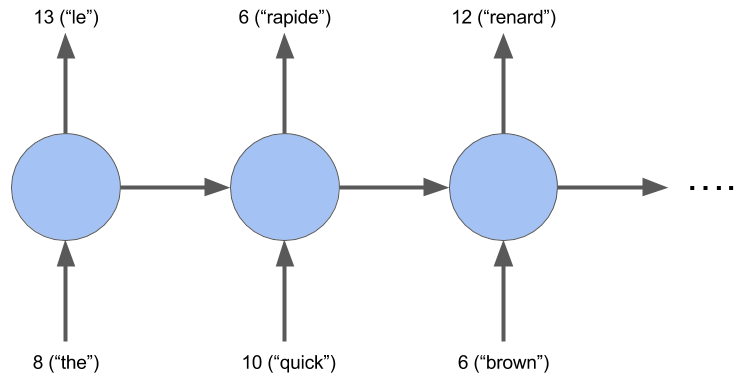
\includegraphics{images/rnn.png} A basic RNN model is a good baseline
for sequence data. In this model, you'll build a RNN that translates
English to French.

    \begin{Verbatim}[commandchars=\\\{\}]
{\color{incolor}In [{\color{incolor}17}]:} \PY{k}{def} \PY{n+nf}{simple\PYZus{}model}\PY{p}{(}\PY{n}{input\PYZus{}shape}\PY{p}{,} \PY{n}{output\PYZus{}sequence\PYZus{}length}\PY{p}{,} \PY{n}{english\PYZus{}vocab\PYZus{}size}\PY{p}{,} \PY{n}{french\PYZus{}vocab\PYZus{}size}\PY{p}{)}\PY{p}{:}
             \PY{l+s+sd}{\PYZdq{}\PYZdq{}\PYZdq{}}
         \PY{l+s+sd}{    Build and train a basic RNN on x and y}
         \PY{l+s+sd}{    :param input\PYZus{}shape: Tuple of input shape}
         \PY{l+s+sd}{    :param output\PYZus{}sequence\PYZus{}length: Length of output sequence}
         \PY{l+s+sd}{    :param english\PYZus{}vocab\PYZus{}size: Number of unique English words in the dataset}
         \PY{l+s+sd}{    :param french\PYZus{}vocab\PYZus{}size: Number of unique French words in the dataset}
         \PY{l+s+sd}{    :return: Keras model built, but not trained}
         \PY{l+s+sd}{    \PYZdq{}\PYZdq{}\PYZdq{}}
             \PY{c+c1}{\PYZsh{} TODO: Build the layers}
             \PY{n}{learning\PYZus{}rate} \PY{o}{=} \PY{l+m+mf}{1e\PYZhy{}3}
             
             \PY{n}{input\PYZus{}sequence} \PY{o}{=} \PY{n}{Input}\PY{p}{(}\PY{n}{input\PYZus{}shape}\PY{p}{[}\PY{l+m+mi}{1}\PY{p}{:}\PY{p}{]}\PY{p}{)}
             \PY{n}{rnn} \PY{o}{=} \PY{n}{GRU}\PY{p}{(}\PY{l+m+mi}{256}\PY{p}{,}\PY{n}{return\PYZus{}sequences}\PY{o}{=}\PY{k+kc}{True}\PY{p}{)}\PY{p}{(}\PY{n}{input\PYZus{}sequence}\PY{p}{)}
             \PY{n}{logits} \PY{o}{=} \PY{n}{TimeDistributed}\PY{p}{(}\PY{n}{Dense}\PY{p}{(}\PY{n}{french\PYZus{}vocab\PYZus{}size}\PY{p}{)}\PY{p}{)}\PY{p}{(}\PY{n}{rnn}\PY{p}{)}
             
             \PY{n}{model} \PY{o}{=} \PY{n}{Model}\PY{p}{(}\PY{n}{input\PYZus{}sequence}\PY{p}{,} \PY{n}{Activation}\PY{p}{(}\PY{l+s+s1}{\PYZsq{}}\PY{l+s+s1}{softmax}\PY{l+s+s1}{\PYZsq{}}\PY{p}{)}\PY{p}{(}\PY{n}{logits}\PY{p}{)}\PY{p}{)}
             \PY{n}{model}\PY{o}{.}\PY{n}{compile}\PY{p}{(}\PY{n}{loss}\PY{o}{=}\PY{n}{sparse\PYZus{}categorical\PYZus{}crossentropy}\PY{p}{,}
                           \PY{n}{optimizer}\PY{o}{=}\PY{n}{Adam}\PY{p}{(}\PY{n}{learning\PYZus{}rate}\PY{p}{)}\PY{p}{,}
                           \PY{n}{metrics}\PY{o}{=}\PY{p}{[}\PY{l+s+s1}{\PYZsq{}}\PY{l+s+s1}{accuracy}\PY{l+s+s1}{\PYZsq{}}\PY{p}{]}\PY{p}{)}
             \PY{k}{return} \PY{n}{model}
         \PY{n}{tests}\PY{o}{.}\PY{n}{test\PYZus{}simple\PYZus{}model}\PY{p}{(}\PY{n}{simple\PYZus{}model}\PY{p}{)}
         
         \PY{c+c1}{\PYZsh{} Reshaping the input to work with a basic RNN}
         \PY{n}{tmp\PYZus{}x} \PY{o}{=} \PY{n}{pad}\PY{p}{(}\PY{n}{preproc\PYZus{}english\PYZus{}sentences}\PY{p}{,} \PY{n}{max\PYZus{}french\PYZus{}sequence\PYZus{}length}\PY{p}{)}
         \PY{n}{tmp\PYZus{}x} \PY{o}{=} \PY{n}{tmp\PYZus{}x}\PY{o}{.}\PY{n}{reshape}\PY{p}{(}\PY{p}{(}\PY{o}{\PYZhy{}}\PY{l+m+mi}{1}\PY{p}{,} \PY{n}{preproc\PYZus{}french\PYZus{}sentences}\PY{o}{.}\PY{n}{shape}\PY{p}{[}\PY{o}{\PYZhy{}}\PY{l+m+mi}{2}\PY{p}{]}\PY{p}{,} \PY{l+m+mi}{1}\PY{p}{)}\PY{p}{)}
         
         \PY{c+c1}{\PYZsh{} Train the neural network}
         \PY{n}{simple\PYZus{}rnn\PYZus{}model} \PY{o}{=} \PY{n}{simple\PYZus{}model}\PY{p}{(}
             \PY{n}{tmp\PYZus{}x}\PY{o}{.}\PY{n}{shape}\PY{p}{,}
             \PY{n}{max\PYZus{}french\PYZus{}sequence\PYZus{}length}\PY{p}{,}
             \PY{n}{english\PYZus{}vocab\PYZus{}size}\PY{p}{,}
             \PY{n}{french\PYZus{}vocab\PYZus{}size}\PY{p}{)}
         \PY{n}{simple\PYZus{}rnn\PYZus{}model}\PY{o}{.}\PY{n}{fit}\PY{p}{(}\PY{n}{tmp\PYZus{}x}\PY{p}{,} \PY{n}{preproc\PYZus{}french\PYZus{}sentences}\PY{p}{,} \PY{n}{batch\PYZus{}size}\PY{o}{=}\PY{l+m+mi}{1024}\PY{p}{,} \PY{n}{epochs}\PY{o}{=}\PY{l+m+mi}{10}\PY{p}{,} \PY{n}{validation\PYZus{}split}\PY{o}{=}\PY{l+m+mf}{0.2}\PY{p}{)}
         
         \PY{c+c1}{\PYZsh{} Print prediction(s)}
         \PY{n+nb}{print}\PY{p}{(}\PY{n}{logits\PYZus{}to\PYZus{}text}\PY{p}{(}\PY{n}{simple\PYZus{}rnn\PYZus{}model}\PY{o}{.}\PY{n}{predict}\PY{p}{(}\PY{n}{tmp\PYZus{}x}\PY{p}{[}\PY{p}{:}\PY{l+m+mi}{1}\PY{p}{]}\PY{p}{)}\PY{p}{[}\PY{l+m+mi}{0}\PY{p}{]}\PY{p}{,} \PY{n}{french\PYZus{}tokenizer}\PY{p}{)}\PY{p}{)}
\end{Verbatim}


    \begin{Verbatim}[commandchars=\\\{\}]
Train on 110288 samples, validate on 27573 samples
Epoch 1/10
110288/110288 [==============================] - 12s 104us/step - loss: 2.5551 - acc: 0.4857 - val\_loss: nan - val\_acc: 0.5661
Epoch 2/10
110288/110288 [==============================] - 11s 97us/step - loss: 1.6201 - acc: 0.5904 - val\_loss: nan - val\_acc: 0.6054
Epoch 3/10
110288/110288 [==============================] - 11s 97us/step - loss: 1.4155 - acc: 0.6164 - val\_loss: nan - val\_acc: 0.6307
Epoch 4/10
110288/110288 [==============================] - 11s 97us/step - loss: 1.2992 - acc: 0.6343 - val\_loss: nan - val\_acc: 0.6465
Epoch 5/10
110288/110288 [==============================] - 11s 97us/step - loss: 1.2100 - acc: 0.6493 - val\_loss: nan - val\_acc: 0.6545
Epoch 6/10
110288/110288 [==============================] - 11s 97us/step - loss: 1.1459 - acc: 0.6604 - val\_loss: nan - val\_acc: 0.6631
Epoch 7/10
110288/110288 [==============================] - 11s 97us/step - loss: 1.0975 - acc: 0.6681 - val\_loss: nan - val\_acc: 0.6734
Epoch 8/10
110288/110288 [==============================] - 11s 97us/step - loss: 1.0596 - acc: 0.6735 - val\_loss: nan - val\_acc: 0.6784
Epoch 9/10
110288/110288 [==============================] - 11s 97us/step - loss: 1.0267 - acc: 0.6779 - val\_loss: nan - val\_acc: 0.6790
Epoch 10/10
110288/110288 [==============================] - 11s 97us/step - loss: 0.9984 - acc: 0.6829 - val\_loss: nan - val\_acc: 0.6880
new jersey est parfois calme en mois de il et il est en en <PAD> <PAD> <PAD> <PAD> <PAD> <PAD> <PAD>

    \end{Verbatim}

    \subsubsection{Model 2: Embedding
(IMPLEMENTATION)}\label{model-2-embedding-implementation}

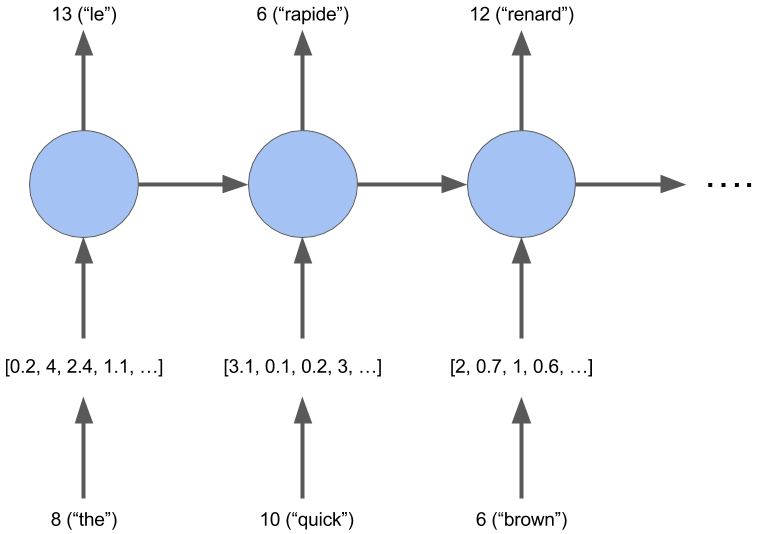
\includegraphics{images/embedding.png} You've turned the words into ids,
but there's a better representation of a word. This is called word
embeddings. An embedding is a vector representation of the word that is
close to similar words in n-dimensional space, where the n represents
the size of the embedding vectors.

In this model, you'll create a RNN model using embedding.

    \begin{Verbatim}[commandchars=\\\{\}]
{\color{incolor}In [{\color{incolor}18}]:} \PY{k}{def} \PY{n+nf}{embed\PYZus{}model}\PY{p}{(}\PY{n}{input\PYZus{}shape}\PY{p}{,} \PY{n}{output\PYZus{}sequence\PYZus{}length}\PY{p}{,} \PY{n}{english\PYZus{}vocab\PYZus{}size}\PY{p}{,} \PY{n}{french\PYZus{}vocab\PYZus{}size}\PY{p}{)}\PY{p}{:}
             \PY{l+s+sd}{\PYZdq{}\PYZdq{}\PYZdq{}}
         \PY{l+s+sd}{    Build and train a RNN model using word embedding on x and y}
         \PY{l+s+sd}{    :param input\PYZus{}shape: Tuple of input shape}
         \PY{l+s+sd}{    :param output\PYZus{}sequence\PYZus{}length: Length of output sequence}
         \PY{l+s+sd}{    :param english\PYZus{}vocab\PYZus{}size: Number of unique English words in the dataset}
         \PY{l+s+sd}{    :param french\PYZus{}vocab\PYZus{}size: Number of unique French words in the dataset}
         \PY{l+s+sd}{    :return: Keras model built, but not trained}
         \PY{l+s+sd}{    \PYZdq{}\PYZdq{}\PYZdq{}}
             \PY{c+c1}{\PYZsh{} TODO: Implement}
             \PY{n}{learning\PYZus{}rate} \PY{o}{=} \PY{l+m+mf}{1e\PYZhy{}3}
             
             \PY{n}{input\PYZus{}sequence} \PY{o}{=} \PY{n}{Input}\PY{p}{(}\PY{n}{input\PYZus{}shape}\PY{p}{[}\PY{l+m+mi}{1}\PY{p}{:}\PY{p}{]}\PY{p}{)}
             \PY{n}{embed\PYZus{}layer} \PY{o}{=} \PY{n}{Embedding}\PY{p}{(}\PY{n}{english\PYZus{}vocab\PYZus{}size}\PY{p}{,} \PY{l+m+mi}{64}\PY{p}{,} \PY{n}{input\PYZus{}length}\PY{o}{=}\PY{n}{output\PYZus{}sequence\PYZus{}length}\PY{p}{)}\PY{p}{(}\PY{n}{input\PYZus{}sequence}\PY{p}{)}
             \PY{n}{rnn} \PY{o}{=} \PY{n}{GRU}\PY{p}{(}\PY{l+m+mi}{128}\PY{p}{,}\PY{n}{return\PYZus{}sequences}\PY{o}{=}\PY{k+kc}{True}\PY{p}{)}\PY{p}{(}\PY{n}{embed\PYZus{}layer}\PY{p}{)}
             \PY{n}{logits} \PY{o}{=} \PY{n}{TimeDistributed}\PY{p}{(}\PY{n}{Dense}\PY{p}{(}\PY{n}{french\PYZus{}vocab\PYZus{}size}\PY{p}{)}\PY{p}{)}\PY{p}{(}\PY{n}{rnn}\PY{p}{)}
             
             \PY{n}{model} \PY{o}{=} \PY{n}{Model}\PY{p}{(}\PY{n}{input\PYZus{}sequence}\PY{p}{,}\PY{n}{Activation}\PY{p}{(}\PY{l+s+s1}{\PYZsq{}}\PY{l+s+s1}{softmax}\PY{l+s+s1}{\PYZsq{}}\PY{p}{)}\PY{p}{(}\PY{n}{logits}\PY{p}{)}\PY{p}{)}
             \PY{n}{model}\PY{o}{.}\PY{n}{compile}\PY{p}{(}\PY{n}{loss} \PY{o}{=} \PY{n}{sparse\PYZus{}categorical\PYZus{}crossentropy}\PY{p}{,}
                          \PY{n}{optimizer} \PY{o}{=} \PY{n}{Adam}\PY{p}{(}\PY{n}{learning\PYZus{}rate}\PY{p}{)}\PY{p}{,}
                          \PY{n}{metrics} \PY{o}{=} \PY{p}{[}\PY{l+s+s1}{\PYZsq{}}\PY{l+s+s1}{accuracy}\PY{l+s+s1}{\PYZsq{}}\PY{p}{]}\PY{p}{)}
             
             \PY{k}{return} \PY{n}{model}
         \PY{n}{tests}\PY{o}{.}\PY{n}{test\PYZus{}embed\PYZus{}model}\PY{p}{(}\PY{n}{embed\PYZus{}model}\PY{p}{)}
         
         
         \PY{c+c1}{\PYZsh{} TODO: Reshape the input}
         \PY{n}{tmp\PYZus{}x} \PY{o}{=} \PY{n}{pad}\PY{p}{(}\PY{n}{preproc\PYZus{}english\PYZus{}sentences}\PY{p}{,} \PY{n}{max\PYZus{}french\PYZus{}sequence\PYZus{}length}\PY{p}{)}
         
         \PY{c+c1}{\PYZsh{} TODO: Train the neural network}
         \PY{n}{embedded\PYZus{}rnn\PYZus{}model} \PY{o}{=} \PY{n}{embed\PYZus{}model}\PY{p}{(}
             \PY{n}{tmp\PYZus{}x}\PY{o}{.}\PY{n}{shape}\PY{p}{,}
             \PY{n}{max\PYZus{}french\PYZus{}sequence\PYZus{}length}\PY{p}{,}
             \PY{n}{english\PYZus{}vocab\PYZus{}size}\PY{p}{,}
             \PY{n}{french\PYZus{}vocab\PYZus{}size}\PY{p}{)}
         \PY{n}{embedded\PYZus{}rnn\PYZus{}model}\PY{o}{.}\PY{n}{fit}\PY{p}{(}\PY{n}{tmp\PYZus{}x}\PY{p}{,} \PY{n}{preproc\PYZus{}french\PYZus{}sentences}\PY{p}{,} \PY{n}{batch\PYZus{}size}\PY{o}{=}\PY{l+m+mi}{1024}\PY{p}{,} \PY{n}{epochs}\PY{o}{=}\PY{l+m+mi}{10}\PY{p}{,} \PY{n}{validation\PYZus{}split}\PY{o}{=}\PY{l+m+mf}{0.2}\PY{p}{)}
         
         \PY{c+c1}{\PYZsh{} TODO: Print prediction(s)}
         \PY{n+nb}{print}\PY{p}{(}\PY{n}{logits\PYZus{}to\PYZus{}text}\PY{p}{(}\PY{n}{embedded\PYZus{}rnn\PYZus{}model}\PY{o}{.}\PY{n}{predict}\PY{p}{(}\PY{n}{tmp\PYZus{}x}\PY{p}{[}\PY{p}{:}\PY{l+m+mi}{1}\PY{p}{]}\PY{p}{)}\PY{p}{[}\PY{l+m+mi}{0}\PY{p}{]}\PY{p}{,} \PY{n}{french\PYZus{}tokenizer}\PY{p}{)}\PY{p}{)}
\end{Verbatim}


    \begin{Verbatim}[commandchars=\\\{\}]
Train on 110288 samples, validate on 27573 samples
Epoch 1/10
110288/110288 [==============================] - 10s 90us/step - loss: 3.4988 - acc: 0.4045 - val\_loss: nan - val\_acc: 0.4229
Epoch 2/10
110288/110288 [==============================] - 9s 81us/step - loss: 2.4239 - acc: 0.4859 - val\_loss: nan - val\_acc: 0.5408
Epoch 3/10
110288/110288 [==============================] - 9s 81us/step - loss: 1.6727 - acc: 0.6041 - val\_loss: nan - val\_acc: 0.6471
Epoch 4/10
110288/110288 [==============================] - 9s 81us/step - loss: 1.2614 - acc: 0.6895 - val\_loss: nan - val\_acc: 0.7321
Epoch 5/10
110288/110288 [==============================] - 9s 81us/step - loss: 1.0038 - acc: 0.7536 - val\_loss: nan - val\_acc: 0.7734
Epoch 6/10
110288/110288 [==============================] - 9s 81us/step - loss: 0.8122 - acc: 0.7895 - val\_loss: nan - val\_acc: 0.8066
Epoch 7/10
110288/110288 [==============================] - 9s 81us/step - loss: 0.6791 - acc: 0.8175 - val\_loss: nan - val\_acc: 0.8292
Epoch 8/10
110288/110288 [==============================] - 9s 81us/step - loss: 0.5914 - acc: 0.8362 - val\_loss: nan - val\_acc: 0.8461
Epoch 9/10
110288/110288 [==============================] - 9s 81us/step - loss: 0.5246 - acc: 0.8517 - val\_loss: nan - val\_acc: 0.8593
Epoch 10/10
110288/110288 [==============================] - 9s 81us/step - loss: 0.4735 - acc: 0.8645 - val\_loss: nan - val\_acc: 0.8702
new jersey est parfois calme en cours de l' il il neige en en <PAD> <PAD> <PAD> <PAD> <PAD> <PAD> <PAD>

    \end{Verbatim}

    \subsubsection{Model 3: Bidirectional RNNs
(IMPLEMENTATION)}\label{model-3-bidirectional-rnns-implementation}

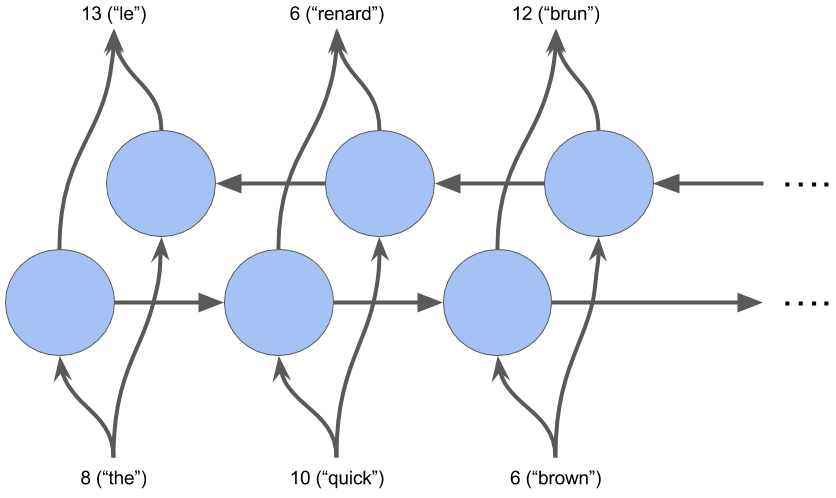
\includegraphics{images/bidirectional.png} One restriction of a RNN is
that it can't see the future input, only the past. This is where
bidirectional recurrent neural networks come in. They are able to see
the future data.

    \begin{Verbatim}[commandchars=\\\{\}]
{\color{incolor}In [{\color{incolor}15}]:} \PY{k}{def} \PY{n+nf}{bd\PYZus{}model}\PY{p}{(}\PY{n}{input\PYZus{}shape}\PY{p}{,} \PY{n}{output\PYZus{}sequence\PYZus{}length}\PY{p}{,} \PY{n}{english\PYZus{}vocab\PYZus{}size}\PY{p}{,} \PY{n}{french\PYZus{}vocab\PYZus{}size}\PY{p}{)}\PY{p}{:}
             \PY{l+s+sd}{\PYZdq{}\PYZdq{}\PYZdq{}}
         \PY{l+s+sd}{    Build and train a bidirectional RNN model on x and y}
         \PY{l+s+sd}{    :param input\PYZus{}shape: Tuple of input shape}
         \PY{l+s+sd}{    :param output\PYZus{}sequence\PYZus{}length: Length of output sequence}
         \PY{l+s+sd}{    :param english\PYZus{}vocab\PYZus{}size: Number of unique English words in the dataset}
         \PY{l+s+sd}{    :param french\PYZus{}vocab\PYZus{}size: Number of unique French words in the dataset}
         \PY{l+s+sd}{    :return: Keras model built, but not trained}
         \PY{l+s+sd}{    \PYZdq{}\PYZdq{}\PYZdq{}}
             \PY{c+c1}{\PYZsh{} TODO: Implement}
             \PY{n}{model} \PY{o}{=} \PY{n}{Sequential}\PY{p}{(}\PY{p}{)}
             \PY{n}{model}\PY{o}{.}\PY{n}{add}\PY{p}{(}\PY{n}{Bidirectional}\PY{p}{(}\PY{n}{GRU}\PY{p}{(}\PY{l+m+mi}{256}\PY{p}{,} \PY{n}{return\PYZus{}sequences}\PY{o}{=}\PY{k+kc}{True}\PY{p}{)}\PY{p}{,} \PY{n}{input\PYZus{}shape}\PY{o}{=}\PY{n}{input\PYZus{}shape}\PY{p}{[}\PY{l+m+mi}{1}\PY{p}{:}\PY{p}{]}\PY{p}{)}\PY{p}{)}
             \PY{n}{model}\PY{o}{.}\PY{n}{add}\PY{p}{(}\PY{n}{TimeDistributed}\PY{p}{(}\PY{n}{Dense}\PY{p}{(}\PY{n}{french\PYZus{}vocab\PYZus{}size}\PY{p}{)}\PY{p}{)}\PY{p}{)}
             \PY{n}{model}\PY{o}{.}\PY{n}{add}\PY{p}{(}\PY{n}{Activation}\PY{p}{(}\PY{l+s+s1}{\PYZsq{}}\PY{l+s+s1}{softmax}\PY{l+s+s1}{\PYZsq{}}\PY{p}{)}\PY{p}{)}
             
             \PY{n}{learning\PYZus{}rate} \PY{o}{=} \PY{l+m+mf}{1e\PYZhy{}3}
             
             \PY{n}{model}\PY{o}{.}\PY{n}{compile}\PY{p}{(}\PY{n}{loss}\PY{o}{=}\PY{n}{sparse\PYZus{}categorical\PYZus{}crossentropy}\PY{p}{,}
                          \PY{n}{optimizer}\PY{o}{=}\PY{n}{Adam}\PY{p}{(}\PY{n}{learning\PYZus{}rate}\PY{p}{)}\PY{p}{,}
                          \PY{n}{metrics}\PY{o}{=}\PY{p}{[}\PY{l+s+s1}{\PYZsq{}}\PY{l+s+s1}{accuracy}\PY{l+s+s1}{\PYZsq{}}\PY{p}{]}\PY{p}{)}
             \PY{k}{return} \PY{n}{model}
         \PY{n}{tests}\PY{o}{.}\PY{n}{test\PYZus{}bd\PYZus{}model}\PY{p}{(}\PY{n}{bd\PYZus{}model}\PY{p}{)}
         
         \PY{c+c1}{\PYZsh{} TODO: Train and Print prediction(s)}
         \PY{n}{tmp\PYZus{}x} \PY{o}{=} \PY{n}{pad}\PY{p}{(}\PY{n}{preproc\PYZus{}english\PYZus{}sentences}\PY{p}{,} \PY{n}{max\PYZus{}french\PYZus{}sequence\PYZus{}length}\PY{p}{)}
         \PY{n}{tmp\PYZus{}x} \PY{o}{=} \PY{n}{tmp\PYZus{}x}\PY{o}{.}\PY{n}{reshape}\PY{p}{(}\PY{p}{(}\PY{o}{\PYZhy{}}\PY{l+m+mi}{1}\PY{p}{,} \PY{n}{preproc\PYZus{}french\PYZus{}sentences}\PY{o}{.}\PY{n}{shape}\PY{p}{[}\PY{o}{\PYZhy{}}\PY{l+m+mi}{2}\PY{p}{]}\PY{p}{,} \PY{l+m+mi}{1}\PY{p}{)}\PY{p}{)}
         
         \PY{n}{bidirectional\PYZus{}model} \PY{o}{=} \PY{n}{bd\PYZus{}model}\PY{p}{(}
             \PY{n}{tmp\PYZus{}x}\PY{o}{.}\PY{n}{shape}\PY{p}{,}
             \PY{n}{max\PYZus{}french\PYZus{}sequence\PYZus{}length}\PY{p}{,}
             \PY{n}{english\PYZus{}vocab\PYZus{}size}\PY{p}{,}
             \PY{n}{french\PYZus{}vocab\PYZus{}size}\PY{p}{)}
         \PY{n}{bidirectional\PYZus{}model}\PY{o}{.}\PY{n}{fit}\PY{p}{(}\PY{n}{tmp\PYZus{}x}\PY{p}{,} \PY{n}{preproc\PYZus{}french\PYZus{}sentences}\PY{p}{,} \PY{n}{batch\PYZus{}size}\PY{o}{=}\PY{l+m+mi}{1024}\PY{p}{,} \PY{n}{epochs}\PY{o}{=}\PY{l+m+mi}{10}\PY{p}{,} \PY{n}{validation\PYZus{}split}\PY{o}{=}\PY{l+m+mf}{0.2}\PY{p}{)}
         
         \PY{n+nb}{print}\PY{p}{(}\PY{n}{logits\PYZus{}to\PYZus{}text}\PY{p}{(}\PY{n}{bidirectional\PYZus{}model}\PY{o}{.}\PY{n}{predict}\PY{p}{(}\PY{n}{tmp\PYZus{}x}\PY{p}{[}\PY{p}{:}\PY{l+m+mi}{1}\PY{p}{]}\PY{p}{)}\PY{p}{[}\PY{l+m+mi}{0}\PY{p}{]}\PY{p}{,} \PY{n}{french\PYZus{}tokenizer}\PY{p}{)}\PY{p}{)}
\end{Verbatim}


    \begin{Verbatim}[commandchars=\\\{\}]
Train on 110288 samples, validate on 27573 samples
Epoch 1/10
110288/110288 [==============================] - 19s 170us/step - loss: 2.1294 - acc: 0.5516 - val\_loss: nan - val\_acc: 0.6139
Epoch 2/10
110288/110288 [==============================] - 18s 163us/step - loss: 1.3609 - acc: 0.6270 - val\_loss: nan - val\_acc: 0.6466
Epoch 3/10
110288/110288 [==============================] - 18s 163us/step - loss: 1.2075 - acc: 0.6535 - val\_loss: nan - val\_acc: 0.6666
Epoch 4/10
110288/110288 [==============================] - 18s 163us/step - loss: 1.1134 - acc: 0.6738 - val\_loss: nan - val\_acc: 0.6804
Epoch 5/10
110288/110288 [==============================] - 18s 163us/step - loss: 1.0373 - acc: 0.6878 - val\_loss: nan - val\_acc: 0.6923
Epoch 6/10
110288/110288 [==============================] - 18s 163us/step - loss: 0.9823 - acc: 0.6970 - val\_loss: nan - val\_acc: 0.7011
Epoch 7/10
110288/110288 [==============================] - 18s 163us/step - loss: 0.9433 - acc: 0.7026 - val\_loss: nan - val\_acc: 0.7088
Epoch 8/10
110288/110288 [==============================] - 18s 163us/step - loss: 0.9040 - acc: 0.7095 - val\_loss: nan - val\_acc: 0.7141
Epoch 9/10
110288/110288 [==============================] - 18s 163us/step - loss: 0.8707 - acc: 0.7155 - val\_loss: nan - val\_acc: 0.7191
Epoch 10/10
110288/110288 [==============================] - 18s 164us/step - loss: 0.8402 - acc: 0.7220 - val\_loss: nan - val\_acc: 0.7244
new jersey est parfois calme au mois et et et il est en en <PAD> <PAD> <PAD> <PAD> <PAD> <PAD> <PAD>

    \end{Verbatim}

    \subsubsection{Model 4: Encoder-Decoder
(OPTIONAL)}\label{model-4-encoder-decoder-optional}

Time to look at encoder-decoder models. This model is made up of an
encoder and decoder. The encoder creates a matrix representation of the
sentence. The decoder takes this matrix as input and predicts the
translation as output.

Create an encoder-decoder model in the cell below.

    \begin{Verbatim}[commandchars=\\\{\}]
{\color{incolor}In [{\color{incolor}14}]:} \PY{k}{def} \PY{n+nf}{encdec\PYZus{}model}\PY{p}{(}\PY{n}{input\PYZus{}shape}\PY{p}{,} \PY{n}{output\PYZus{}sequence\PYZus{}length}\PY{p}{,} \PY{n}{english\PYZus{}vocab\PYZus{}size}\PY{p}{,} \PY{n}{french\PYZus{}vocab\PYZus{}size}\PY{p}{)}\PY{p}{:}
             \PY{l+s+sd}{\PYZdq{}\PYZdq{}\PYZdq{}}
         \PY{l+s+sd}{    Build and train an encoder\PYZhy{}decoder model on x and y}
         \PY{l+s+sd}{    :param input\PYZus{}shape: Tuple of input shape}
         \PY{l+s+sd}{    :param output\PYZus{}sequence\PYZus{}length: Length of output sequence}
         \PY{l+s+sd}{    :param english\PYZus{}vocab\PYZus{}size: Number of unique English words in the dataset}
         \PY{l+s+sd}{    :param french\PYZus{}vocab\PYZus{}size: Number of unique French words in the dataset}
         \PY{l+s+sd}{    :return: Keras model built, but not trained}
         \PY{l+s+sd}{    \PYZdq{}\PYZdq{}\PYZdq{}}
             \PY{c+c1}{\PYZsh{} OPTIONAL: Implement}
             \PY{c+c1}{\PYZsh{} encoder input model}
             \PY{n}{model} \PY{o}{=} \PY{n}{Sequential}\PY{p}{(}\PY{p}{)}
             \PY{n}{model}\PY{o}{.}\PY{n}{add}\PY{p}{(}\PY{n}{LSTM}\PY{p}{(}\PY{l+m+mi}{256}\PY{p}{,} \PY{n}{input\PYZus{}shape} \PY{o}{=} \PY{n}{input\PYZus{}shape}\PY{p}{[}\PY{l+m+mi}{1}\PY{p}{:}\PY{p}{]}\PY{p}{,} \PY{n}{go\PYZus{}backwards} \PY{o}{=} \PY{k+kc}{True}\PY{p}{,} \PY{n}{name}\PY{o}{=}\PY{l+s+s2}{\PYZdq{}}\PY{l+s+s2}{encoder1}\PY{l+s+s2}{\PYZdq{}}\PY{p}{)}\PY{p}{)}
             \PY{n}{model}\PY{o}{.}\PY{n}{add}\PY{p}{(}\PY{n}{RepeatVector}\PY{p}{(}\PY{n}{output\PYZus{}sequence\PYZus{}length}\PY{p}{,} \PY{n}{name}\PY{o}{=}\PY{l+s+s2}{\PYZdq{}}\PY{l+s+s2}{encoder2}\PY{l+s+s2}{\PYZdq{}}\PY{p}{)}\PY{p}{)}
             
             \PY{c+c1}{\PYZsh{} decoder output model}
             \PY{n}{model}\PY{o}{.}\PY{n}{add}\PY{p}{(}\PY{n}{LSTM}\PY{p}{(}\PY{l+m+mi}{256}\PY{p}{,} \PY{n}{return\PYZus{}sequences}\PY{o}{=}\PY{k+kc}{True}\PY{p}{,} \PY{n}{name}\PY{o}{=}\PY{l+s+s2}{\PYZdq{}}\PY{l+s+s2}{decoder}\PY{l+s+s2}{\PYZdq{}}\PY{p}{)}\PY{p}{)}
             \PY{n}{model}\PY{o}{.}\PY{n}{add}\PY{p}{(}\PY{n}{TimeDistributed}\PY{p}{(}\PY{n}{Dense}\PY{p}{(}\PY{n}{french\PYZus{}vocab\PYZus{}size}\PY{p}{)}\PY{p}{,} \PY{n}{name}\PY{o}{=}\PY{l+s+s2}{\PYZdq{}}\PY{l+s+s2}{logits}\PY{l+s+s2}{\PYZdq{}}\PY{p}{)}\PY{p}{)}
             \PY{n}{model}\PY{o}{.}\PY{n}{add}\PY{p}{(}\PY{n}{Activation}\PY{p}{(}\PY{l+s+s1}{\PYZsq{}}\PY{l+s+s1}{softmax}\PY{l+s+s1}{\PYZsq{}}\PY{p}{,} \PY{n}{name}\PY{o}{=}\PY{l+s+s1}{\PYZsq{}}\PY{l+s+s1}{activation}\PY{l+s+s1}{\PYZsq{}}\PY{p}{)}\PY{p}{)}
             
             \PY{c+c1}{\PYZsh{}Building the model}
             \PY{n}{learning\PYZus{}rate} \PY{o}{=} \PY{l+m+mf}{1e\PYZhy{}3}
             \PY{n}{model}\PY{o}{.}\PY{n}{compile}\PY{p}{(}\PY{n}{loss} \PY{o}{=} \PY{l+s+s1}{\PYZsq{}}\PY{l+s+s1}{sparse\PYZus{}categorical\PYZus{}crossentropy}\PY{l+s+s1}{\PYZsq{}}\PY{p}{,}
                          \PY{n}{optimizer} \PY{o}{=} \PY{n}{Adam}\PY{p}{(}\PY{n}{learning\PYZus{}rate}\PY{p}{)}\PY{p}{,}
                          \PY{n}{metrics} \PY{o}{=} \PY{p}{[}\PY{l+s+s1}{\PYZsq{}}\PY{l+s+s1}{accuracy}\PY{l+s+s1}{\PYZsq{}}\PY{p}{]}\PY{p}{)}
             \PY{k}{return} \PY{n}{model}
         
         \PY{n}{tests}\PY{o}{.}\PY{n}{test\PYZus{}encdec\PYZus{}model}\PY{p}{(}\PY{n}{encdec\PYZus{}model}\PY{p}{)}
         
         
         \PY{c+c1}{\PYZsh{} OPTIONAL: Train and Print prediction(s)}
         \PY{n}{tmp\PYZus{}x} \PY{o}{=} \PY{n}{pad}\PY{p}{(}\PY{n}{preproc\PYZus{}english\PYZus{}sentences}\PY{p}{,} \PY{n}{preproc\PYZus{}french\PYZus{}sentences}\PY{o}{.}\PY{n}{shape}\PY{p}{[}\PY{l+m+mi}{1}\PY{p}{]}\PY{p}{)}
         \PY{n}{tmp\PYZus{}x} \PY{o}{=} \PY{n}{tmp\PYZus{}x}\PY{o}{.}\PY{n}{reshape}\PY{p}{(}\PY{p}{(}\PY{o}{\PYZhy{}}\PY{l+m+mi}{1}\PY{p}{,} \PY{n}{preproc\PYZus{}french\PYZus{}sentences}\PY{o}{.}\PY{n}{shape}\PY{p}{[}\PY{o}{\PYZhy{}}\PY{l+m+mi}{2}\PY{p}{]}\PY{p}{,} \PY{l+m+mi}{1}\PY{p}{)}\PY{p}{)}
         
         \PY{n}{ed\PYZus{}model} \PY{o}{=} \PY{n}{encdec\PYZus{}model}\PY{p}{(}
             \PY{n}{tmp\PYZus{}x}\PY{o}{.}\PY{n}{shape}\PY{p}{,}
             \PY{n}{max\PYZus{}french\PYZus{}sequence\PYZus{}length}\PY{p}{,}
             \PY{n}{english\PYZus{}vocab\PYZus{}size}\PY{p}{,}
             \PY{n}{french\PYZus{}vocab\PYZus{}size}\PY{p}{)}
         \PY{n}{ed\PYZus{}model}\PY{o}{.}\PY{n}{fit}\PY{p}{(}\PY{n}{tmp\PYZus{}x}\PY{p}{,} \PY{n}{preproc\PYZus{}french\PYZus{}sentences}\PY{p}{,} \PY{n}{batch\PYZus{}size}\PY{o}{=}\PY{l+m+mi}{1024}\PY{p}{,} \PY{n}{epochs}\PY{o}{=}\PY{l+m+mi}{10}\PY{p}{,} \PY{n}{validation\PYZus{}split}\PY{o}{=}\PY{l+m+mf}{0.2}\PY{p}{)}
         
         \PY{n+nb}{print}\PY{p}{(}\PY{n}{logits\PYZus{}to\PYZus{}text}\PY{p}{(}\PY{n}{ed\PYZus{}model}\PY{o}{.}\PY{n}{predict}\PY{p}{(}\PY{n}{tmp\PYZus{}x}\PY{p}{[}\PY{p}{:}\PY{l+m+mi}{1}\PY{p}{]}\PY{p}{)}\PY{p}{[}\PY{l+m+mi}{0}\PY{p}{]}\PY{p}{,} \PY{n}{french\PYZus{}tokenizer}\PY{p}{)}\PY{p}{)}
\end{Verbatim}


    \begin{Verbatim}[commandchars=\\\{\}]
Train on 110288 samples, validate on 27573 samples
Epoch 1/10
110288/110288 [==============================] - 27s 243us/step - loss: 2.7456 - acc: 0.4562 - val\_loss: nan - val\_acc: 0.5080
Epoch 2/10
110288/110288 [==============================] - 24s 220us/step - loss: 1.8934 - acc: 0.5473 - val\_loss: nan - val\_acc: 0.5842
Epoch 3/10
110288/110288 [==============================] - 24s 220us/step - loss: 1.5519 - acc: 0.5956 - val\_loss: nan - val\_acc: 0.6122
Epoch 4/10
110288/110288 [==============================] - 24s 221us/step - loss: 1.4046 - acc: 0.6175 - val\_loss: nan - val\_acc: 0.6261
Epoch 5/10
110288/110288 [==============================] - 24s 220us/step - loss: 1.3205 - acc: 0.6298 - val\_loss: nan - val\_acc: 0.6373
Epoch 6/10
110288/110288 [==============================] - 24s 221us/step - loss: 1.2641 - acc: 0.6392 - val\_loss: nan - val\_acc: 0.6440
Epoch 7/10
110288/110288 [==============================] - 24s 220us/step - loss: 1.2178 - acc: 0.6493 - val\_loss: nan - val\_acc: 0.6512
Epoch 8/10
110288/110288 [==============================] - 24s 221us/step - loss: 1.1605 - acc: 0.6625 - val\_loss: nan - val\_acc: 0.6631
Epoch 9/10
110288/110288 [==============================] - 24s 220us/step - loss: 1.1000 - acc: 0.6756 - val\_loss: nan - val\_acc: 0.6628
Epoch 10/10
110288/110288 [==============================] - 24s 221us/step - loss: 1.0516 - acc: 0.6842 - val\_loss: nan - val\_acc: 0.6930
new jersey est généralement pluvieux en l' et il est il en en <PAD> <PAD> <PAD> <PAD> <PAD> <PAD> <PAD> <PAD>

    \end{Verbatim}

    \subsubsection{Model 5: Custom
(IMPLEMENTATION)}\label{model-5-custom-implementation}

Use everything you learned from the previous models to create a model
that incorporates embedding and a bidirectional rnn into one model.

    \begin{Verbatim}[commandchars=\\\{\}]
{\color{incolor}In [{\color{incolor}29}]:} \PY{k}{def} \PY{n+nf}{model\PYZus{}final}\PY{p}{(}\PY{n}{input\PYZus{}shape}\PY{p}{,} \PY{n}{output\PYZus{}sequence\PYZus{}length}\PY{p}{,} \PY{n}{english\PYZus{}vocab\PYZus{}size}\PY{p}{,} \PY{n}{french\PYZus{}vocab\PYZus{}size}\PY{p}{)}\PY{p}{:}
             \PY{l+s+sd}{\PYZdq{}\PYZdq{}\PYZdq{}}
         \PY{l+s+sd}{    Build and train a model that incorporates embedding, encoder\PYZhy{}decoder, and bidirectional RNN on x and y}
         \PY{l+s+sd}{    :param input\PYZus{}shape: Tuple of input shape}
         \PY{l+s+sd}{    :param output\PYZus{}sequence\PYZus{}length: Length of output sequence}
         \PY{l+s+sd}{    :param english\PYZus{}vocab\PYZus{}size: Number of unique English words in the dataset}
         \PY{l+s+sd}{    :param french\PYZus{}vocab\PYZus{}size: Number of unique French words in the dataset}
         \PY{l+s+sd}{    :return: Keras model built, but not trained}
         \PY{l+s+sd}{    \PYZdq{}\PYZdq{}\PYZdq{}}
             \PY{c+c1}{\PYZsh{} TODO: Implement}
             \PY{n}{model} \PY{o}{=} \PY{n}{Sequential}\PY{p}{(}\PY{p}{)}
             \PY{n}{model}\PY{o}{.}\PY{n}{add}\PY{p}{(}\PY{n}{Embedding}\PY{p}{(}\PY{n}{english\PYZus{}vocab\PYZus{}size}\PY{p}{,} \PY{l+m+mi}{256}\PY{p}{,} \PY{n}{input\PYZus{}length} \PY{o}{=} \PY{n}{input\PYZus{}shape}\PY{p}{[}\PY{l+m+mi}{1}\PY{p}{]}\PY{p}{)}\PY{p}{)}
             \PY{n}{model}\PY{o}{.}\PY{n}{add}\PY{p}{(}\PY{n}{Bidirectional}\PY{p}{(}\PY{n}{LSTM}\PY{p}{(}\PY{l+m+mi}{256}\PY{p}{)}\PY{p}{)}\PY{p}{)}
             
             \PY{c+c1}{\PYZsh{} encoder input layer}
             \PY{n}{model}\PY{o}{.}\PY{n}{add}\PY{p}{(}\PY{n}{RepeatVector}\PY{p}{(}\PY{n}{output\PYZus{}sequence\PYZus{}length}\PY{p}{)}\PY{p}{)}
             
             \PY{c+c1}{\PYZsh{} decoder output model}
             \PY{n}{model}\PY{o}{.}\PY{n}{add}\PY{p}{(}\PY{n}{LSTM}\PY{p}{(}\PY{l+m+mi}{256}\PY{p}{,} \PY{n}{return\PYZus{}sequences}\PY{o}{=}\PY{k+kc}{True}\PY{p}{)}\PY{p}{)}
             
             \PY{n}{model}\PY{o}{.}\PY{n}{add}\PY{p}{(}\PY{n}{TimeDistributed}\PY{p}{(}\PY{n}{Dense}\PY{p}{(}\PY{n}{french\PYZus{}vocab\PYZus{}size}\PY{p}{)}\PY{p}{)}\PY{p}{)}
             \PY{n}{model}\PY{o}{.}\PY{n}{add}\PY{p}{(}\PY{n}{Activation}\PY{p}{(}\PY{l+s+s1}{\PYZsq{}}\PY{l+s+s1}{softmax}\PY{l+s+s1}{\PYZsq{}}\PY{p}{)}\PY{p}{)}
             
             \PY{c+c1}{\PYZsh{}Compiling the model}
             \PY{n}{learning\PYZus{}rate} \PY{o}{=} \PY{l+m+mf}{1e\PYZhy{}3}
             \PY{n}{model}\PY{o}{.}\PY{n}{compile}\PY{p}{(}\PY{n}{loss} \PY{o}{=} \PY{l+s+s1}{\PYZsq{}}\PY{l+s+s1}{sparse\PYZus{}categorical\PYZus{}crossentropy}\PY{l+s+s1}{\PYZsq{}}\PY{p}{,}
                          \PY{n}{optimizer} \PY{o}{=} \PY{n}{Adam}\PY{p}{(}\PY{n}{learning\PYZus{}rate}\PY{p}{)}\PY{p}{,}
                          \PY{n}{metrics} \PY{o}{=} \PY{p}{[}\PY{l+s+s1}{\PYZsq{}}\PY{l+s+s1}{accuracy}\PY{l+s+s1}{\PYZsq{}}\PY{p}{]}\PY{p}{)}
             \PY{k}{return} \PY{n}{model}
         \PY{n}{tests}\PY{o}{.}\PY{n}{test\PYZus{}model\PYZus{}final}\PY{p}{(}\PY{n}{model\PYZus{}final}\PY{p}{)}
         
         
         \PY{n+nb}{print}\PY{p}{(}\PY{l+s+s1}{\PYZsq{}}\PY{l+s+s1}{Final Model Loaded}\PY{l+s+s1}{\PYZsq{}}\PY{p}{)}
         \PY{c+c1}{\PYZsh{} TODO: Train the final model}
         \PY{n}{tmp\PYZus{}x} \PY{o}{=} \PY{n}{pad}\PY{p}{(}\PY{n}{preproc\PYZus{}english\PYZus{}sentences}\PY{p}{,} \PY{n}{preproc\PYZus{}french\PYZus{}sentences}\PY{o}{.}\PY{n}{shape}\PY{p}{[}\PY{l+m+mi}{1}\PY{p}{]}\PY{p}{)}
         
         \PY{n}{combo\PYZus{}model} \PY{o}{=} \PY{n}{model\PYZus{}final}\PY{p}{(}
             \PY{n}{tmp\PYZus{}x}\PY{o}{.}\PY{n}{shape}\PY{p}{,}
             \PY{n}{max\PYZus{}french\PYZus{}sequence\PYZus{}length}\PY{p}{,}
             \PY{n}{english\PYZus{}vocab\PYZus{}size}\PY{p}{,}
             \PY{n}{french\PYZus{}vocab\PYZus{}size}\PY{p}{)}
         \PY{n}{combo\PYZus{}model}\PY{o}{.}\PY{n}{fit}\PY{p}{(}\PY{n}{tmp\PYZus{}x}\PY{p}{,} \PY{n}{preproc\PYZus{}french\PYZus{}sentences}\PY{p}{,} \PY{n}{batch\PYZus{}size}\PY{o}{=}\PY{l+m+mi}{1024}\PY{p}{,} \PY{n}{epochs}\PY{o}{=}\PY{l+m+mi}{10}\PY{p}{,} \PY{n}{validation\PYZus{}split}\PY{o}{=}\PY{l+m+mf}{0.2}\PY{p}{)}
\end{Verbatim}


    \begin{Verbatim}[commandchars=\\\{\}]
Final Model Loaded
Train on 110288 samples, validate on 27573 samples
Epoch 1/10
110288/110288 [==============================] - 35s 322us/step - loss: 2.8425 - acc: 0.4434 - val\_loss: nan - val\_acc: 0.5063
Epoch 2/10
110288/110288 [==============================] - 33s 303us/step - loss: 1.8661 - acc: 0.5371 - val\_loss: nan - val\_acc: 0.5717
Epoch 3/10
110288/110288 [==============================] - 33s 303us/step - loss: 1.5141 - acc: 0.6106 - val\_loss: nan - val\_acc: 0.6374
Epoch 4/10
110288/110288 [==============================] - 33s 303us/step - loss: 1.2979 - acc: 0.6529 - val\_loss: nan - val\_acc: 0.6732
Epoch 5/10
110288/110288 [==============================] - 33s 303us/step - loss: 1.1198 - acc: 0.6895 - val\_loss: nan - val\_acc: 0.7051
Epoch 6/10
110288/110288 [==============================] - 33s 303us/step - loss: 0.9900 - acc: 0.7172 - val\_loss: nan - val\_acc: 0.7267
Epoch 7/10
110288/110288 [==============================] - 33s 303us/step - loss: 0.9121 - acc: 0.7338 - val\_loss: nan - val\_acc: 0.7432
Epoch 8/10
110288/110288 [==============================] - 33s 303us/step - loss: 0.8429 - acc: 0.7507 - val\_loss: nan - val\_acc: 0.7582
Epoch 9/10
110288/110288 [==============================] - 33s 303us/step - loss: 0.7816 - acc: 0.7669 - val\_loss: nan - val\_acc: 0.7773
Epoch 10/10
110288/110288 [==============================] - 33s 303us/step - loss: 0.7187 - acc: 0.7844 - val\_loss: nan - val\_acc: 0.7922

    \end{Verbatim}

\begin{Verbatim}[commandchars=\\\{\}]
{\color{outcolor}Out[{\color{outcolor}29}]:} <keras.callbacks.History at 0x7ff50e5ddef0>
\end{Verbatim}
            
    \subsection{Prediction
(IMPLEMENTATION)}\label{prediction-implementation}

    \begin{Verbatim}[commandchars=\\\{\}]
{\color{incolor}In [{\color{incolor}30}]:} \PY{k}{def} \PY{n+nf}{final\PYZus{}predictions}\PY{p}{(}\PY{n}{x}\PY{p}{,} \PY{n}{y}\PY{p}{,} \PY{n}{x\PYZus{}tk}\PY{p}{,} \PY{n}{y\PYZus{}tk}\PY{p}{)}\PY{p}{:}
             \PY{l+s+sd}{\PYZdq{}\PYZdq{}\PYZdq{}}
         \PY{l+s+sd}{    Gets predictions using the final model}
         \PY{l+s+sd}{    :param x: Preprocessed English data}
         \PY{l+s+sd}{    :param y: Preprocessed French data}
         \PY{l+s+sd}{    :param x\PYZus{}tk: English tokenizer}
         \PY{l+s+sd}{    :param y\PYZus{}tk: French tokenizer}
         \PY{l+s+sd}{    \PYZdq{}\PYZdq{}\PYZdq{}}
             \PY{c+c1}{\PYZsh{} TODO: Train neural network using model\PYZus{}final}
             \PY{n}{tmp\PYZus{}x} \PY{o}{=} \PY{n}{pad}\PY{p}{(}\PY{n}{x}\PY{p}{)}
             \PY{n}{model} \PY{o}{=} \PY{n}{model\PYZus{}final}\PY{p}{(}\PY{n}{tmp\PYZus{}x}\PY{o}{.}\PY{n}{shape}\PY{p}{,}
                                 \PY{n}{max\PYZus{}french\PYZus{}sequence\PYZus{}length}\PY{p}{,}
                                 \PY{n}{english\PYZus{}vocab\PYZus{}size} \PY{o}{+} \PY{l+m+mi}{1}\PY{p}{,}
                                 \PY{n}{french\PYZus{}vocab\PYZus{}size} \PY{o}{+} \PY{l+m+mi}{1}\PY{p}{)}
             \PY{n}{model}\PY{o}{.}\PY{n}{fit}\PY{p}{(}\PY{n}{tmp\PYZus{}x}\PY{p}{,} \PY{n}{y}\PY{p}{,} \PY{n}{batch\PYZus{}size}\PY{o}{=}\PY{l+m+mi}{1024}\PY{p}{,} \PY{n}{epochs}\PY{o}{=}\PY{l+m+mi}{20}\PY{p}{,} \PY{n}{validation\PYZus{}split}\PY{o}{=}\PY{l+m+mf}{0.2}\PY{p}{)}
         
             
             \PY{c+c1}{\PYZsh{}\PYZsh{} DON\PYZsq{}T EDIT ANYTHING BELOW THIS LINE}
             \PY{n}{y\PYZus{}id\PYZus{}to\PYZus{}word} \PY{o}{=} \PY{p}{\PYZob{}}\PY{n}{value}\PY{p}{:} \PY{n}{key} \PY{k}{for} \PY{n}{key}\PY{p}{,} \PY{n}{value} \PY{o+ow}{in} \PY{n}{y\PYZus{}tk}\PY{o}{.}\PY{n}{word\PYZus{}index}\PY{o}{.}\PY{n}{items}\PY{p}{(}\PY{p}{)}\PY{p}{\PYZcb{}}
             \PY{n}{y\PYZus{}id\PYZus{}to\PYZus{}word}\PY{p}{[}\PY{l+m+mi}{0}\PY{p}{]} \PY{o}{=} \PY{l+s+s1}{\PYZsq{}}\PY{l+s+s1}{\PYZlt{}PAD\PYZgt{}}\PY{l+s+s1}{\PYZsq{}}
         
             \PY{n}{sentence} \PY{o}{=} \PY{l+s+s1}{\PYZsq{}}\PY{l+s+s1}{he saw a old yellow truck}\PY{l+s+s1}{\PYZsq{}}
             \PY{n}{sentence} \PY{o}{=} \PY{p}{[}\PY{n}{x\PYZus{}tk}\PY{o}{.}\PY{n}{word\PYZus{}index}\PY{p}{[}\PY{n}{word}\PY{p}{]} \PY{k}{for} \PY{n}{word} \PY{o+ow}{in} \PY{n}{sentence}\PY{o}{.}\PY{n}{split}\PY{p}{(}\PY{p}{)}\PY{p}{]}
             \PY{n}{sentence} \PY{o}{=} \PY{n}{pad\PYZus{}sequences}\PY{p}{(}\PY{p}{[}\PY{n}{sentence}\PY{p}{]}\PY{p}{,} \PY{n}{maxlen}\PY{o}{=}\PY{n}{x}\PY{o}{.}\PY{n}{shape}\PY{p}{[}\PY{o}{\PYZhy{}}\PY{l+m+mi}{1}\PY{p}{]}\PY{p}{,} \PY{n}{padding}\PY{o}{=}\PY{l+s+s1}{\PYZsq{}}\PY{l+s+s1}{post}\PY{l+s+s1}{\PYZsq{}}\PY{p}{)}
             \PY{n}{sentences} \PY{o}{=} \PY{n}{np}\PY{o}{.}\PY{n}{array}\PY{p}{(}\PY{p}{[}\PY{n}{sentence}\PY{p}{[}\PY{l+m+mi}{0}\PY{p}{]}\PY{p}{,} \PY{n}{x}\PY{p}{[}\PY{l+m+mi}{0}\PY{p}{]}\PY{p}{]}\PY{p}{)}
             \PY{n}{predictions} \PY{o}{=} \PY{n}{model}\PY{o}{.}\PY{n}{predict}\PY{p}{(}\PY{n}{sentences}\PY{p}{,} \PY{n+nb}{len}\PY{p}{(}\PY{n}{sentences}\PY{p}{)}\PY{p}{)}
         
             \PY{n+nb}{print}\PY{p}{(}\PY{l+s+s1}{\PYZsq{}}\PY{l+s+s1}{Sample 1:}\PY{l+s+s1}{\PYZsq{}}\PY{p}{)}
             \PY{n+nb}{print}\PY{p}{(}\PY{l+s+s1}{\PYZsq{}}\PY{l+s+s1}{ }\PY{l+s+s1}{\PYZsq{}}\PY{o}{.}\PY{n}{join}\PY{p}{(}\PY{p}{[}\PY{n}{y\PYZus{}id\PYZus{}to\PYZus{}word}\PY{p}{[}\PY{n}{np}\PY{o}{.}\PY{n}{argmax}\PY{p}{(}\PY{n}{x}\PY{p}{)}\PY{p}{]} \PY{k}{for} \PY{n}{x} \PY{o+ow}{in} \PY{n}{predictions}\PY{p}{[}\PY{l+m+mi}{0}\PY{p}{]}\PY{p}{]}\PY{p}{)}\PY{p}{)}
             \PY{n+nb}{print}\PY{p}{(}\PY{l+s+s1}{\PYZsq{}}\PY{l+s+s1}{Il a vu un vieux camion jaune}\PY{l+s+s1}{\PYZsq{}}\PY{p}{)}
             \PY{n+nb}{print}\PY{p}{(}\PY{l+s+s1}{\PYZsq{}}\PY{l+s+s1}{Sample 2:}\PY{l+s+s1}{\PYZsq{}}\PY{p}{)}
             \PY{n+nb}{print}\PY{p}{(}\PY{l+s+s1}{\PYZsq{}}\PY{l+s+s1}{ }\PY{l+s+s1}{\PYZsq{}}\PY{o}{.}\PY{n}{join}\PY{p}{(}\PY{p}{[}\PY{n}{y\PYZus{}id\PYZus{}to\PYZus{}word}\PY{p}{[}\PY{n}{np}\PY{o}{.}\PY{n}{argmax}\PY{p}{(}\PY{n}{x}\PY{p}{)}\PY{p}{]} \PY{k}{for} \PY{n}{x} \PY{o+ow}{in} \PY{n}{predictions}\PY{p}{[}\PY{l+m+mi}{1}\PY{p}{]}\PY{p}{]}\PY{p}{)}\PY{p}{)}
             \PY{n+nb}{print}\PY{p}{(}\PY{l+s+s1}{\PYZsq{}}\PY{l+s+s1}{ }\PY{l+s+s1}{\PYZsq{}}\PY{o}{.}\PY{n}{join}\PY{p}{(}\PY{p}{[}\PY{n}{y\PYZus{}id\PYZus{}to\PYZus{}word}\PY{p}{[}\PY{n}{np}\PY{o}{.}\PY{n}{max}\PY{p}{(}\PY{n}{x}\PY{p}{)}\PY{p}{]} \PY{k}{for} \PY{n}{x} \PY{o+ow}{in} \PY{n}{y}\PY{p}{[}\PY{l+m+mi}{0}\PY{p}{]}\PY{p}{]}\PY{p}{)}\PY{p}{)}
         
         
         \PY{n}{final\PYZus{}predictions}\PY{p}{(}\PY{n}{preproc\PYZus{}english\PYZus{}sentences}\PY{p}{,} \PY{n}{preproc\PYZus{}french\PYZus{}sentences}\PY{p}{,} \PY{n}{english\PYZus{}tokenizer}\PY{p}{,} \PY{n}{french\PYZus{}tokenizer}\PY{p}{)}
\end{Verbatim}


    \begin{Verbatim}[commandchars=\\\{\}]
Train on 110288 samples, validate on 27573 samples
Epoch 1/20
110288/110288 [==============================] - 31s 279us/step - loss: 2.8283 - acc: 0.4479 - val\_loss: 2.0654 - val\_acc: 0.4995
Epoch 2/20
110288/110288 [==============================] - 29s 259us/step - loss: 1.8757 - acc: 0.5313 - val\_loss: 1.6689 - val\_acc: 0.5718
Epoch 3/20
110288/110288 [==============================] - 29s 260us/step - loss: 1.5245 - acc: 0.6030 - val\_loss: 1.4386 - val\_acc: 0.6231
Epoch 4/20
110288/110288 [==============================] - 29s 260us/step - loss: 1.3240 - acc: 0.6460 - val\_loss: 1.2320 - val\_acc: 0.6650
Epoch 5/20
110288/110288 [==============================] - 29s 260us/step - loss: 1.1482 - acc: 0.6834 - val\_loss: 1.0679 - val\_acc: 0.7003
Epoch 6/20
110288/110288 [==============================] - 29s 260us/step - loss: 1.0132 - acc: 0.7116 - val\_loss: 0.9642 - val\_acc: 0.7211
Epoch 7/20
110288/110288 [==============================] - 29s 260us/step - loss: 0.9256 - acc: 0.7306 - val\_loss: 0.8928 - val\_acc: 0.7388
Epoch 8/20
110288/110288 [==============================] - 29s 260us/step - loss: 0.8588 - acc: 0.7478 - val\_loss: 0.8089 - val\_acc: 0.7625
Epoch 9/20
110288/110288 [==============================] - 29s 260us/step - loss: 0.7768 - acc: 0.7709 - val\_loss: 0.7543 - val\_acc: 0.7786
Epoch 10/20
110288/110288 [==============================] - 29s 260us/step - loss: 0.7145 - acc: 0.7902 - val\_loss: 0.6812 - val\_acc: 0.8001
Epoch 11/20
110288/110288 [==============================] - 29s 260us/step - loss: 0.6463 - acc: 0.8103 - val\_loss: 0.6274 - val\_acc: 0.8170
Epoch 12/20
110288/110288 [==============================] - 29s 260us/step - loss: 0.5889 - acc: 0.8282 - val\_loss: 0.5584 - val\_acc: 0.8378
Epoch 13/20
110288/110288 [==============================] - 29s 260us/step - loss: 0.5287 - acc: 0.8471 - val\_loss: 0.5069 - val\_acc: 0.8545
Epoch 14/20
110288/110288 [==============================] - 29s 260us/step - loss: 0.4772 - acc: 0.8628 - val\_loss: 0.4633 - val\_acc: 0.8680
Epoch 15/20
110288/110288 [==============================] - 29s 260us/step - loss: 0.4276 - acc: 0.8798 - val\_loss: 0.4048 - val\_acc: 0.8888
Epoch 16/20
110288/110288 [==============================] - 29s 260us/step - loss: 0.3757 - acc: 0.8978 - val\_loss: 0.3614 - val\_acc: 0.9023
Epoch 17/20
110288/110288 [==============================] - 29s 260us/step - loss: 0.3293 - acc: 0.9131 - val\_loss: 0.3195 - val\_acc: 0.9164
Epoch 18/20
110288/110288 [==============================] - 29s 260us/step - loss: 0.2920 - acc: 0.9248 - val\_loss: 0.3348 - val\_acc: 0.9131
Epoch 19/20
110288/110288 [==============================] - 29s 260us/step - loss: 0.2572 - acc: 0.9358 - val\_loss: 0.2537 - val\_acc: 0.9371
Epoch 20/20
110288/110288 [==============================] - 29s 260us/step - loss: 0.2257 - acc: 0.9444 - val\_loss: 0.2320 - val\_acc: 0.9426
Sample 1:
il a vu un vieux camion jaune <PAD> <PAD> <PAD> <PAD> <PAD> <PAD> <PAD> <PAD> <PAD> <PAD> <PAD> <PAD> <PAD> <PAD>
Il a vu un vieux camion jaune
Sample 2:
new jersey est parfois calme pendant l' automne il il est neigeux en avril <PAD> <PAD> <PAD> <PAD> <PAD> <PAD> <PAD>
new jersey est parfois calme pendant l' automne et il est neigeux en avril <PAD> <PAD> <PAD> <PAD> <PAD> <PAD> <PAD>

    \end{Verbatim}

    \subsection{Submission}\label{submission}

When you're ready to submit, complete the following steps: 1. Review the
\href{https://review.udacity.com/\#!/rubrics/1004/view}{rubric} to
ensure your submission meets all requirements to pass 2. Generate an
HTML version of this notebook

\begin{itemize}
\item
  Run the next cell to attempt automatic generation (this is the
  recommended method in Workspaces)
\item
  Navigate to \textbf{FILE -\textgreater{} Download as -\textgreater{}
  HTML (.html)}
\item
  Manually generate a copy using \texttt{nbconvert} from your shell
  terminal

\begin{verbatim}
$ pip install nbconvert
$ python -m nbconvert machine_translation.ipynb
\end{verbatim}
\end{itemize}

\begin{enumerate}
\def\labelenumi{\arabic{enumi}.}
\setcounter{enumi}{2}
\tightlist
\item
  Submit the project
\end{enumerate}

\begin{itemize}
\item
  If you are in a Workspace, simply click the "Submit Project" button
  (bottom towards the right)
\item
  Otherwise, add the following files into a zip archive and submit them
\item
  \texttt{helper.py}
\item
  \texttt{machine\_translation.ipynb}
\item
  \texttt{machine\_translation.html}

  \begin{itemize}
  \tightlist
  \item
    You can export the notebook by navigating to \textbf{File
    -\textgreater{} Download as -\textgreater{} HTML (.html)}.
  \end{itemize}
\end{itemize}

    \subsubsection{Generate the html}\label{generate-the-html}

\textbf{Save your notebook before running the next cell to generate the
HTML output.} Then submit your project.

    \begin{Verbatim}[commandchars=\\\{\}]
{\color{incolor}In [{\color{incolor}2}]:} \PY{c+c1}{\PYZsh{} Save before you run this cell!}
        \PY{o}{!!}jupyter nbconvert *.ipynb
\end{Verbatim}


\begin{Verbatim}[commandchars=\\\{\}]
{\color{outcolor}Out[{\color{outcolor}2}]:} ['[NbConvertApp] Converting notebook machine\_translation.ipynb to html',
         '[NbConvertApp] Writing 305996 bytes to machine\_translation.html']
\end{Verbatim}
            
    \subsection{Optional Enhancements}\label{optional-enhancements}

This project focuses on learning various network architectures for
machine translation, but we don't evaluate the models according to best
practices by splitting the data into separate test \& training sets -\/-
so the model accuracy is overstated. Use the
\href{http://scikit-learn.org/stable/modules/generated/sklearn.model_selection.train_test_split.html}{\texttt{sklearn.model\_selection.train\_test\_split()}}
function to create separate training \& test datasets, then retrain each
of the models using only the training set and evaluate the prediction
accuracy using the hold out test set. Does the "best" model change?


    % Add a bibliography block to the postdoc
    
    
    
    \end{document}
